%%%%%%%%%%%%%%%%%%%%%%%%%%%%%%%%%%%%%%%%%
% The Legrand Orange Book
% LaTeX Template
% Version 2.1.1 (14/2/16)
%
% This template has been downloaded from:
% http://www.LaTeXTemplates.com
%
% Original author:
% Mathias Legrand (legrand.mathias@gmail.com) with modifications by:
% Vel (vel@latextemplates.com)
%
% License:
% CC BY-NC-SA 3.0 (http://creativecommons.org/licenses/by-nc-sa/3.0/)
%
% Compiling this template:
% This template uses biber for its bibliography and makeindex for its index.
% When you first open the template, compile it from the command line with the 
% commands below to make sure your LaTeX distribution is configured correctly:
%
% 1) pdflatex main
% 2) makeindex main.idx -s StyleInd.ist
% 3) biber main
% 4) pdflatex main x 2
%
% After this, when you wish to update the bibliography/index use the appropriate
% command above and make sure to compile with pdflatex several times 
% afterwards to propagate your changes to the document.
%
% This template also uses a number of packages which may need to be
% updated to the newest versions for the template to compile. It is strongly
% recommended you update your LaTeX distribution if you have any
% compilation errors.
%
% Important note:
% Chapter heading images should have a 2:1 width:height ratio,
% e.g. 920px width and 460px height.
%
%%%%%%%%%%%%%%%%%%%%%%%%%%%%%%%%%%%%%%%%%

%----------------------------------------------------------------------------------------
%	PACKAGES AND OTHER DOCUMENT CONFIGURATIONS
%----------------------------------------------------------------------------------------

\documentclass[11pt,fleqn]{book} % Default font size and left-justified equations

%----------------------------------------------------------------------------------------

%%%%%%%%%%%%%%%%%%%%%%%%%%%%%%%%%%%%%%%%%
% The Legrand Orange Book
% Structural Definitions File
% Version 2.0 (9/2/15)
%
% Original author:
% Mathias Legrand (legrand.mathias@gmail.com) with modifications by:
% Vel (vel@latextemplates.com)
% 
% This file has been downloaded from:
% http://www.LaTeXTemplates.com
%
% License:
% CC BY-NC-SA 3.0 (http://creativecommons.org/licenses/by-nc-sa/3.0/)
%
%%%%%%%%%%%%%%%%%%%%%%%%%%%%%%%%%%%%%%%%%

%----------------------------------------------------------------------------------------
%	VARIOUS REQUIRED PACKAGES AND CONFIGURATIONS
%----------------------------------------------------------------------------------------

\usepackage[top=3cm,bottom=3cm,left=3cm,right=3cm,headsep=10pt,a4paper]{geometry} % Page margins

\usepackage{graphicx} % Required for including pictures
\graphicspath{{Pictures/}} % Specifies the directory where pictures are stored

\usepackage{lipsum} % Inserts dummy text

\usepackage{tikz} % Required for drawing custom shapes

\usepackage[spanish]{babel} % English language/hyphenation

\usepackage{enumitem} % Customize lists
\setlist{nolistsep} % Reduce spacing between bullet points and numbered lists

\usepackage{booktabs} % Required for nicer horizontal rules in tables

\usepackage{xcolor} % Required for specifying colors by name
\definecolor{ocre}{RGB}{243,102,25} % Define the orange color used for highlighting throughout the book
\usepackage{cancel}%Para números tachados
\usepackage{subfig}%Para poner imágenes paralelas

%----------------------------------------------------------------------------------------
%	FONTS
%----------------------------------------------------------------------------------------

\usepackage{avant} % Use the Avantgarde font for headings
%\usepackage{times} % Use the Times font for headings
\usepackage{mathptmx} % Use the Adobe Times Roman as the default text font together with math symbols from the Sym­bol, Chancery and Com­puter Modern fonts

\usepackage{microtype} % Slightly tweak font spacing for aesthetics
\usepackage[utf8]{inputenc} % Required for including letters with accents
\usepackage[T1]{fontenc} % Use 8-bit encoding that has 256 glyphs

%----------------------------------------------------------------------------------------
%	BIBLIOGRAPHY AND INDEX
%----------------------------------------------------------------------------------------

\usepackage[style=alphabetic,citestyle=numeric,sorting=nyt,sortcites=true,autopunct=true,babel=hyphen,hyperref=true,abbreviate=false,backref=true,backend=biber]{biblatex}
\addbibresource{bibliography.bib} % BibTeX bibliography file
\defbibheading{bibempty}{}

\usepackage{calc} % For simpler calculation - used for spacing the index letter headings correctly
\usepackage{makeidx} % Required to make an index
\makeindex % Tells LaTeX to create the files required for indexing

%----------------------------------------------------------------------------------------
%	MAIN TABLE OF CONTENTS
%----------------------------------------------------------------------------------------

\usepackage{titletoc} % Required for manipulating the table of contents

\contentsmargin{0cm} % Removes the default margin

% Part text styling
\titlecontents{part}[0cm]
{\addvspace{20pt}\centering\large\bfseries}
{}
{}
{}

% Chapter text styling
\titlecontents{chapter}[1.25cm] % Indentation
{\addvspace{12pt}\large\sffamily\bfseries} % Spacing and font options for chapters
{\color{ocre!60}\contentslabel[\Large\thecontentslabel]{1.25cm}\color{ocre}} % Chapter number
{\color{ocre}}  
{\color{ocre!60}\normalsize\;\titlerule*[.5pc]{.}\;\thecontentspage} % Page number

% Section text styling
\titlecontents{section}[1.25cm] % Indentation
{\addvspace{3pt}\sffamily\bfseries} % Spacing and font options for sections
{\contentslabel[\thecontentslabel]{1.25cm}} % Section number
{}
{\hfill\color{black}\thecontentspage} % Page number
[]

% Subsection text styling
\titlecontents{subsection}[1.25cm] % Indentation
{\addvspace{1pt}\sffamily\small} % Spacing and font options for subsections
{\contentslabel[\thecontentslabel]{1.25cm}} % Subsection number
{}
{\ \titlerule*[.5pc]{.}\;\thecontentspage} % Page number
[]

% List of figures
\titlecontents{figure}[0em]
{\addvspace{-5pt}\sffamily}
{\thecontentslabel\hspace*{1em}}
{}
{\ \titlerule*[.5pc]{.}\;\thecontentspage}
[]

% List of tables
\titlecontents{table}[0em]
{\addvspace{-5pt}\sffamily}
{\thecontentslabel\hspace*{1em}}
{}
{\ \titlerule*[.5pc]{.}\;\thecontentspage}
[]

%----------------------------------------------------------------------------------------
%	MINI TABLE OF CONTENTS IN PART HEADS
%----------------------------------------------------------------------------------------

% Chapter text styling
\titlecontents{lchapter}[0em] % Indenting
{\addvspace{15pt}\large\sffamily\bfseries} % Spacing and font options for chapters
{\color{ocre}\contentslabel[\Large\thecontentslabel]{1.25cm}\color{ocre}} % Chapter number
{}  
{\color{ocre}\normalsize\sffamily\bfseries\;\titlerule*[.5pc]{.}\;\thecontentspage} % Page number

% Section text styling
\titlecontents{lsection}[0em] % Indenting
{\sffamily\small} % Spacing and font options for sections
{\contentslabel[\thecontentslabel]{1.25cm}} % Section number
{}
{}

% Subsection text styling
\titlecontents{lsubsection}[.5em] % Indentation
{\normalfont\footnotesize\sffamily} % Font settings
{}
{}
{}

%----------------------------------------------------------------------------------------
%	PAGE HEADERS
%----------------------------------------------------------------------------------------

\usepackage{fancyhdr} % Required for header and footer configuration

\pagestyle{fancy}
\renewcommand{\chaptermark}[1]{\markboth{\sffamily\normalsize\bfseries\chaptername\ \thechapter.\ #1}{}} % Chapter text font settings
\renewcommand{\sectionmark}[1]{\markright{\sffamily\normalsize\thesection\hspace{5pt}#1}{}} % Section text font settings
\fancyhf{} \fancyhead[LE,RO]{\sffamily\normalsize\thepage} % Font setting for the page number in the header
\fancyhead[LO]{\rightmark} % Print the nearest section name on the left side of odd pages
\fancyhead[RE]{\leftmark} % Print the current chapter name on the right side of even pages
\renewcommand{\headrulewidth}{0.5pt} % Width of the rule under the header
\addtolength{\headheight}{2.5pt} % Increase the spacing around the header slightly
\renewcommand{\footrulewidth}{0pt} % Removes the rule in the footer
\fancypagestyle{plain}{\fancyhead{}\renewcommand{\headrulewidth}{0pt}} % Style for when a plain pagestyle is specified

% Removes the header from odd empty pages at the end of chapters
\makeatletter
\renewcommand{\cleardoublepage}{
\clearpage\ifodd\c@page\else
\hbox{}
\vspace*{\fill}
\thispagestyle{empty}
\newpage
\fi}

%----------------------------------------------------------------------------------------
%	THEOREM STYLES
%----------------------------------------------------------------------------------------

\usepackage{amsmath,amsfonts,amssymb,amsthm} % For math equations, theorems, symbols, etc

\newcommand{\intoo}[2]{\mathopen{]}#1\,;#2\mathclose{[}}
\newcommand{\ud}{\mathop{\mathrm{{}d}}\mathopen{}}
\newcommand{\intff}[2]{\mathopen{[}#1\,;#2\mathclose{]}}
\newtheorem{notation}{Notation}[chapter]

% Boxed/framed environments
\newtheoremstyle{ocrenumbox}% % Theorem style name
{0pt}% Space above
{0pt}% Space below
{\normalfont}% % Body font
{}% Indent amount
{\small\bf\sffamily\color{ocre}}% % Theorem head font
{\;}% Punctuation after theorem head
{0.25em}% Space after theorem head
{\small\sffamily\color{ocre}\thmname{#1}\nobreakspace\thmnumber{\@ifnotempty{#1}{}\@upn{#2}}% Theorem text (e.g. Theorem 2.1)
\thmnote{\nobreakspace\the\thm@notefont\sffamily\bfseries\color{black}---\nobreakspace#3.}} % Optional theorem note
\renewcommand{\qedsymbol}{$\blacksquare$}% Optional qed square

\newtheoremstyle{blacknumex}% Theorem style name
{5pt}% Space above
{5pt}% Space below
{\normalfont}% Body font
{} % Indent amount
{\small\bf\sffamily}% Theorem head font
{\;}% Punctuation after theorem head
{0.25em}% Space after theorem head
{\small\sffamily{\tiny\ensuremath{\blacksquare}}\nobreakspace\thmname{#1}\nobreakspace\thmnumber{\@ifnotempty{#1}{}\@upn{#2}}% Theorem text (e.g. Theorem 2.1)
\thmnote{\nobreakspace\the\thm@notefont\sffamily\bfseries---\nobreakspace#3.}}% Optional theorem note

\newtheoremstyle{blacknumbox} % Theorem style name
{0pt}% Space above
{0pt}% Space below
{\normalfont}% Body font
{}% Indent amount
{\small\bf\sffamily}% Theorem head font
{\;}% Punctuation after theorem head
{0.25em}% Space after theorem head
{\small\sffamily\thmname{#1}\nobreakspace\thmnumber{\@ifnotempty{#1}{}\@upn{#2}}% Theorem text (e.g. Theorem 2.1)
\thmnote{\nobreakspace\the\thm@notefont\sffamily\bfseries---\nobreakspace#3.}}% Optional theorem note

% Non-boxed/non-framed environments
\newtheoremstyle{ocrenum}% % Theorem style name
{5pt}% Space above
{5pt}% Space below
{\normalfont}% % Body font
{}% Indent amount
{\small\bf\sffamily\color{ocre}}% % Theorem head font
{\;}% Punctuation after theorem head
{0.25em}% Space after theorem head
{\small\sffamily\color{ocre}\thmname{#1}\nobreakspace\thmnumber{\@ifnotempty{#1}{}\@upn{#2}}% Theorem text (e.g. Theorem 2.1)
\thmnote{\nobreakspace\the\thm@notefont\sffamily\bfseries\color{black}---\nobreakspace#3.}} % Optional theorem note
\renewcommand{\qedsymbol}{$\blacksquare$}% Optional qed square
\makeatother

% Defines the theorem text style for each type of theorem to one of the three styles above
\newcounter{dummy} 
\numberwithin{dummy}{section}
\theoremstyle{ocrenumbox}
\newtheorem{theoremeT}[dummy]{Theorem}
\newtheorem{problem}{Problema}[chapter]
\newtheorem{exerciseT}{Exercise}[chapter]
\theoremstyle{blacknumex}
\newtheorem{exampleT}{Example}[chapter]
\theoremstyle{blacknumbox}
\newtheorem{vocabulary}{Vocabulary}[chapter]
\newtheorem{definitionT}{Definition}[section]
\newtheorem{corollaryT}[dummy]{Corollary}
\theoremstyle{ocrenum}
\newtheorem{proposition}[dummy]{Proposition}

%----------------------------------------------------------------------------------------
%	DEFINITION OF COLORED BOXES
%----------------------------------------------------------------------------------------

\RequirePackage[framemethod=default]{mdframed} % Required for creating the theorem, definition, exercise and corollary boxes

% Theorem box
\newmdenv[skipabove=7pt,
skipbelow=7pt,
backgroundcolor=black!5,
linecolor=ocre,
innerleftmargin=5pt,
innerrightmargin=5pt,
innertopmargin=5pt,
leftmargin=0cm,
rightmargin=0cm,
innerbottommargin=5pt]{tBox}

% Exercise box	  
\newmdenv[skipabove=7pt,
skipbelow=7pt,
rightline=false,
leftline=true,
topline=false,
bottomline=false,
backgroundcolor=ocre!10,
linecolor=ocre,
innerleftmargin=5pt,
innerrightmargin=5pt,
innertopmargin=5pt,
innerbottommargin=5pt,
leftmargin=0cm,
rightmargin=0cm,
linewidth=4pt]{eBox}	

% Definition box
\newmdenv[skipabove=7pt,
skipbelow=7pt,
rightline=false,
leftline=true,
topline=false,
bottomline=false,
linecolor=ocre,
innerleftmargin=5pt,
innerrightmargin=5pt,
innertopmargin=0pt,
leftmargin=0cm,
rightmargin=0cm,
linewidth=4pt,
innerbottommargin=0pt]{dBox}	

% Corollary box
\newmdenv[skipabove=7pt,
skipbelow=7pt,
rightline=false,
leftline=true,
topline=false,
bottomline=false,
linecolor=gray,
backgroundcolor=black!5,
innerleftmargin=5pt,
innerrightmargin=5pt,
innertopmargin=5pt,
leftmargin=0cm,
rightmargin=0cm,
linewidth=4pt,
innerbottommargin=5pt]{cBox}

% Creates an environment for each type of theorem and assigns it a theorem text style from the "Theorem Styles" section above and a colored box from above
\newenvironment{theorem}{\begin{tBox}\begin{theoremeT}}{\end{theoremeT}\end{tBox}}
\newenvironment{exercise}{\begin{eBox}\begin{exerciseT}}{\hfill{\color{ocre}\tiny\ensuremath{\blacksquare}}\end{exerciseT}\end{eBox}}				  
\newenvironment{definition}{\begin{dBox}\begin{definitionT}}{\end{definitionT}\end{dBox}}	
\newenvironment{example}{\begin{exampleT}}{\hfill{\tiny\ensuremath{\blacksquare}}\end{exampleT}}		
\newenvironment{corollary}{\begin{cBox}\begin{corollaryT}}{\end{corollaryT}\end{cBox}}	

%----------------------------------------------------------------------------------------
%	REMARK ENVIRONMENT
%----------------------------------------------------------------------------------------

\newenvironment{remark}{\par\vspace{10pt}\small % Vertical white space above the remark and smaller font size
\begin{list}{}{
\leftmargin=35pt % Indentation on the left
\rightmargin=25pt}\item\ignorespaces % Indentation on the right
\makebox[-2.5pt]{\begin{tikzpicture}[overlay]
\node[draw=ocre!60,line width=1pt,circle,fill=ocre!25,font=\sffamily\bfseries,inner sep=2pt,outer sep=0pt] at (-15pt,0pt){\textcolor{ocre}{R}};\end{tikzpicture}} % Orange R in a circle
\advance\baselineskip -1pt}{\end{list}\vskip5pt} % Tighter line spacing and white space after remark

%----------------------------------------------------------------------------------------
%	SECTION NUMBERING IN THE MARGIN
%----------------------------------------------------------------------------------------

\makeatletter
\renewcommand{\@seccntformat}[1]{\llap{\textcolor{ocre}{\csname the#1\endcsname}\hspace{1em}}}                    
\renewcommand{\section}{\@startsection{section}{1}{\z@}
{-4ex \@plus -1ex \@minus -.4ex}
{1ex \@plus.2ex }
{\normalfont\large\sffamily\bfseries}}
\renewcommand{\subsection}{\@startsection {subsection}{2}{\z@}
{-3ex \@plus -0.1ex \@minus -.4ex}
{0.5ex \@plus.2ex }
{\normalfont\sffamily\bfseries}}
\renewcommand{\subsubsection}{\@startsection {subsubsection}{3}{\z@}
{-2ex \@plus -0.1ex \@minus -.2ex}
{.2ex \@plus.2ex }
{\normalfont\small\sffamily\bfseries}}                        
\renewcommand\paragraph{\@startsection{paragraph}{4}{\z@}
{-2ex \@plus-.2ex \@minus .2ex}
{.1ex}
{\normalfont\small\sffamily\bfseries}}

%----------------------------------------------------------------------------------------
%	PART HEADINGS
%----------------------------------------------------------------------------------------

% numbered part in the table of contents
\newcommand{\@mypartnumtocformat}[2]{%
\setlength\fboxsep{0pt}%
\noindent\colorbox{ocre!20}{\strut\parbox[c][.7cm]{\ecart}{\color{ocre!70}\Large\sffamily\bfseries\centering#1}}\hskip\esp\colorbox{ocre!40}{\strut\parbox[c][.7cm]{\linewidth-\ecart-\esp}{\Large\sffamily\centering#2}}}%
%%%%%%%%%%%%%%%%%%%%%%%%%%%%%%%%%%
% unnumbered part in the table of contents
\newcommand{\@myparttocformat}[1]{%
\setlength\fboxsep{0pt}%
\noindent\colorbox{ocre!40}{\strut\parbox[c][.7cm]{\linewidth}{\Large\sffamily\centering#1}}}%
%%%%%%%%%%%%%%%%%%%%%%%%%%%%%%%%%%
\newlength\esp
\setlength\esp{4pt}
\newlength\ecart
\setlength\ecart{1.2cm-\esp}
\newcommand{\thepartimage}{}%
\newcommand{\partimage}[1]{\renewcommand{\thepartimage}{#1}}%
\def\@part[#1]#2{%
\ifnum \c@secnumdepth >-2\relax%
\refstepcounter{part}%
\addcontentsline{toc}{part}{\texorpdfstring{\protect\@mypartnumtocformat{\thepart}{#1}}{\partname~\thepart\ ---\ #1}}
\else%
\addcontentsline{toc}{part}{\texorpdfstring{\protect\@myparttocformat{#1}}{#1}}%
\fi%
\startcontents%
\markboth{}{}%
{\thispagestyle{empty}%
\begin{tikzpicture}[remember picture,overlay]%
\node at (current page.north west){\begin{tikzpicture}[remember picture,overlay]%	
\fill[ocre!20](0cm,0cm) rectangle (\paperwidth,-\paperheight);
\node[anchor=north] at (4cm,-3.25cm){\color{ocre!40}\fontsize{220}{100}\sffamily\bfseries\@Roman\c@part}; 
\node[anchor=south east] at (\paperwidth-1cm,-\paperheight+1cm){\parbox[t][][t]{8.5cm}{
\printcontents{l}{0}{\setcounter{tocdepth}{1}}%
}};
\node[anchor=north east] at (\paperwidth-1.5cm,-3.25cm){\parbox[t][][t]{15cm}{\strut\raggedleft\color{white}\fontsize{30}{30}\sffamily\bfseries#2}};
\end{tikzpicture}};
\end{tikzpicture}}%
\@endpart}
\def\@spart#1{%
\startcontents%
\phantomsection
{\thispagestyle{empty}%
\begin{tikzpicture}[remember picture,overlay]%
\node at (current page.north west){\begin{tikzpicture}[remember picture,overlay]%	
\fill[ocre!20](0cm,0cm) rectangle (\paperwidth,-\paperheight);
\node[anchor=north east] at (\paperwidth-1.5cm,-3.25cm){\parbox[t][][t]{15cm}{\strut\raggedleft\color{white}\fontsize{30}{30}\sffamily\bfseries#1}};
\end{tikzpicture}};
\end{tikzpicture}}
\addcontentsline{toc}{part}{\texorpdfstring{%
\setlength\fboxsep{0pt}%
\noindent\protect\colorbox{ocre!40}{\strut\protect\parbox[c][.7cm]{\linewidth}{\Large\sffamily\protect\centering #1\quad\mbox{}}}}{#1}}%
\@endpart}
\def\@endpart{\vfil\newpage
\if@twoside
\if@openright
\null
\thispagestyle{empty}%
\newpage
\fi
\fi
\if@tempswa
\twocolumn
\fi}

%----------------------------------------------------------------------------------------
%	CHAPTER HEADINGS
%----------------------------------------------------------------------------------------

% A switch to conditionally include a picture, implemented by  Christian Hupfer
\newif\ifusechapterimage
\usechapterimagetrue
\newcommand{\thechapterimage}{}%
\newcommand{\chapterimage}[1]{\ifusechapterimage\renewcommand{\thechapterimage}{#1}\fi}%
\def\@makechapterhead#1{%
{\parindent \z@ \raggedright \normalfont
\ifnum \c@secnumdepth >\m@ne
\if@mainmatter
\begin{tikzpicture}[remember picture,overlay]
\node at (current page.north west)
{\begin{tikzpicture}[remember picture,overlay]
\node[anchor=north west,inner sep=0pt] at (0,0) {\ifusechapterimage\includegraphics[width=\paperwidth]{\thechapterimage}\fi};
\draw[anchor=west] (\Gm@lmargin,-9cm) node [line width=2pt,rounded corners=15pt,draw=ocre,fill=white,fill opacity=0.5,inner sep=15pt]{\strut\makebox[22cm]{}};
\draw[anchor=west] (\Gm@lmargin+.3cm,-9cm) node {\huge\sffamily\bfseries\color{black}\thechapter. #1\strut};
\end{tikzpicture}};
\end{tikzpicture}
\else
\begin{tikzpicture}[remember picture,overlay]
\node at (current page.north west)
{\begin{tikzpicture}[remember picture,overlay]
\node[anchor=north west,inner sep=0pt] at (0,0) {\ifusechapterimage\includegraphics[width=\paperwidth]{\thechapterimage}\fi};
\draw[anchor=west] (\Gm@lmargin,-9cm) node [line width=2pt,rounded corners=15pt,draw=ocre,fill=white,fill opacity=0.5,inner sep=15pt]{\strut\makebox[22cm]{}};
\draw[anchor=west] (\Gm@lmargin+.3cm,-9cm) node {\huge\sffamily\bfseries\color{black}#1\strut};
\end{tikzpicture}};
\end{tikzpicture}
\fi\fi\par\vspace*{270\p@}}}

%-------------------------------------------

\def\@makeschapterhead#1{%
\begin{tikzpicture}[remember picture,overlay]
\node at (current page.north west)
{\begin{tikzpicture}[remember picture,overlay]
\node[anchor=north west,inner sep=0pt] at (0,0) {\ifusechapterimage\includegraphics[width=\paperwidth]{\thechapterimage}\fi};
\draw[anchor=west] (\Gm@lmargin,-9cm) node [line width=2pt,rounded corners=15pt,draw=ocre,fill=white,fill opacity=0.5,inner sep=15pt]{\strut\makebox[22cm]{}};
\draw[anchor=west] (\Gm@lmargin+.3cm,-9cm) node {\huge\sffamily\bfseries\color{black}#1\strut};
\end{tikzpicture}};
\end{tikzpicture}
\par\vspace*{270\p@}}
\makeatother

%----------------------------------------------------------------------------------------
%	HYPERLINKS IN THE DOCUMENTS
%----------------------------------------------------------------------------------------

\usepackage{hyperref}
\hypersetup{hidelinks,backref=true,pagebackref=true,hyperindex=true,colorlinks=false,breaklinks=true,urlcolor= ocre,bookmarks=true,bookmarksopen=false,pdftitle={Title},pdfauthor={Author}}
\usepackage{bookmark}
\bookmarksetup{
open,
numbered,
addtohook={%
\ifnum\bookmarkget{level}=0 % chapter
\bookmarksetup{bold}%
\fi
\ifnum\bookmarkget{level}=-1 % part
\bookmarksetup{color=ocre,bold}%
\fi
}
}
 % Insert the commands.tex file which contains the majority of the structure behind the template

\begin{document}
%----------------------------------------------------------------------------------------

\newcounter{nx}%Contador para las listas de reglas orgánicas. Capitulo 2.

%----------------------------------------------------------------------------------------
%	TITLE PAGE
%----------------------------------------------------------------------------------------

\begingroup
\thispagestyle{empty}
\begin{tikzpicture}[remember picture,overlay]
\coordinate [below=12cm] (midpoint) at (current page.north);
\node at (current page.north west)
{\begin{tikzpicture}[remember picture,overlay]
\node[anchor=north west,inner sep=0pt] at (0,0) {
\includegraphics[width=\paperwidth]{background}}; % Background image
\draw[anchor=north] (midpoint) node [fill=ocre!30!white,fill opacity=0.6,text opacity=1,inner sep=1cm]{\Huge\centering\bfseries\sffamily\parbox[c][][t]{\paperwidth}{\centering Química para Segundo de Bachillerato\\[15pt] % Book title
{\Large Apuntes para uso en clase}\\[20pt] % Subtitle
{\huge Javier Perán Jódar}}}; % Author name
\end{tikzpicture}};
\end{tikzpicture}
\vfill
\endgroup

%----------------------------------------------------------------------------------------
%	COPYRIGHT PAGE
%----------------------------------------------------------------------------------------

\newpage
~\vfill
\thispagestyle{empty}

\noindent Copyright \copyright\ 2013 John Smith\\ % Copyright notice

\noindent \textsc{Published by Publisher}\\ % Publisher

\noindent \textsc{book-website.com}\\ % URL

\noindent Licensed under the Creative Commons Attribution-NonCommercial 3.0 Unported License (the ``License''). You may not use this file except in compliance with the License. You may obtain a copy of the License at \url{http://creativecommons.org/licenses/by-nc/3.0}. Unless required by applicable law or agreed to in writing, software distributed under the License is distributed on an \textsc{``as is'' basis, without warranties or conditions of any kind}, either express or implied. See the License for the specific language governing permissions and limitations under the License.\\ % License information

\noindent \textit{First printing, March 2013} % Printing/edition date

%----------------------------------------------------------------------------------------
%	TABLE OF CONTENTS
%----------------------------------------------------------------------------------------

%\usechapterimagefalse % If you don't want to include a chapter image, use this to toggle images off - it can be enabled later with \usechapterimagetrue

\chapterimage{chapter_head_1.pdf} % Table of contents heading image

\pagestyle{empty} % No headers

\tableofcontents % Print the table of contents itself

\cleardoublepage % Forces the first chapter to start on an odd page so it's on the right

\pagestyle{fancy} % Print headers again

%----------------------------------------------------------------------------------------
%	PART
%----------------------------------------------------------------------------------------

\part{Formulación Química}

%----------------------------------------------------------------------------------------
%	CHAPTER 1
%----------------------------------------------------------------------------------------

\chapterimage{chapter_head_2.pdf} % Chapter heading image

\chapter{Formulación en Química Inorgánica}

\section{Introducción}\index{Paragraphs of Text}
Desde los primeros albores de las ciencias químicas, los científicos han buscado un método de nomenclatura capaz de representar y reflejar la complejidad y diversidad de la materia que forma el mundo físico que nos rodea. Así, partiendo de los primeros trabajos al respecto del científico inglés \emph{J. Dalton (1766-1844)} los sistemas de nomenclatura han ido evolucionando a la par que la propia química, e igual que cualquier lengua, se han adaptado a los nuevos cambios y descubrimientos, y a la manera en que los propios químicos han desarrollado una ciencia con poco mas de 200 años de historia.\\
En 1919 se crea la \emph{International Union of Pure and Applied Chemistry (IUPAC)} como organismo internacional para, entre otros cometidos, establecer estándares globales de simbología y protocolos operacionales en química.Por tanto, hoy en día la IUPAC es la máxima autoridad en materia de nomenclatura química, y es la encargada de revisar e introducir los cambios pertinentes en los distintos sistemas según el desarrollo natural de la propia ciencia.\\

La última revisión de los protocolos de nomenclatura y formulación tuvo lugar en el año 2005, y fueron publicados, para el caso de la formulación inorgánica, en el “Libro Rojo de la IUPAC” de 2007. Este capítulo contiene todas las nuevas modalidades de nomenclatura y formulación. que incluyen cambios radicales en la manera de nombrar oxoácidos, oxisales y oxoaniones. Como todos los cambios de especial envergadura en ciencia requieren de un periodo de adaptación, se han incluido en los anexos la nomenclatura de dichas especies mediante los sistemas anteriores a las recomendaciones de 2005, de forma que el alumno pueda comprenderlos en el caso de que alguna publicación todavía los contenga.

\section{Sistemas de Nomenclatura}
En el desarrollo de la nomenclatura química han surgido varios sistemas para la construcción de los nombres de los elementos y compuestos químicos. Cada uno de los sistemas tiene su propio conjunto de reglas.
Algunos sistemas son de aplicación general; en cambio, otros han surgido de la necesidad de usar sistemas más especializados en áreas determinadas de la química.
En concreto, en lo referente a la química inorgánica, tres son los sistemas principales de nomenclatura: la nomenclatura de composición, la de sustitución y la de adición.
La nomenclatura de adición es quizás la que puede usarse de forma más generalizada en química inorgánica. La nomenclatura de sustitución puede usarse en determinadas áreas. Estos dos sistemas requieren el conocimiento de la estructura de las especies químicas que van a ser nombradas. En cambio, la nomenclatura de composición puede usarse cuando no es necesario aportar información sobre la estructura de las sustancias, o no se conoce, y sólo se indica la estequiometría o composición.

\subsection{Nomenclatura de Composición}
Esta nomenclatura está basada en la composición no en la estructura. Por ello, puede ser la única forma de nombrar un compuesto si no se dispone de información estructural.\\
El tipo más simple de este tipo de nomenclatura es la llamada estequiométrica. En ella se indica la proporción de los constituyentes a partir de la fórmula empírica o la molecular. La proporción de los elementos o constituyentes puede indicarse de varias formas:\\
\begin{itemize}
	\item Utilizando prefijos multiplicativos (Método Sistemático). 
	\item Utilizando números de oxidación de los elementos (Sistema de Stock, mediante números romanos). 
	\item Utilizando la carga de los iones (mediante los números de Ewens-Basset, números arábigos seguido del signo correspondiente)
\end{itemize}
\subsection{Nomenclatura de Sustitución}
De forma general, en esta nomenclatura se parte del nombre de unos compuestos denominados Hidruros Parentales y se indica, junto con los prefijos de cantidad correspondientes, el nombre de los elementos o grupos que sustituyen a los hidrógenos. Esta nomenclatura es la usada generalmente para nombrar los compuestos orgánicos.
\subsection{Nomenclatura de Adición}
Esta nomenclatura se desarrolló originalmente para nombrar los compuestos de coordinación. Así, se considera que el compuesto consta de un átomo central o átomos centrales con ligandos asociados, cuyo número se indica con los prefijos multiplicativos correspondientes.\\
Los tres sistemas de nomenclatura pueden proporcionar nombres diferentes, pero sin  ambigüedades, para un compuesto dado. La elección entre los tres sistemas depende de la clase de compuesto inorgánico que se trate y el grado de detalle que se desea comunicar.
\section{Tipos de Nomenclatura más utilizados}
A continuación pasaremos a detallar los tipos de nomenclatura mas empleados en Química Inorgánica, independientemente que estos sistemas sean de Composición, Sustitución o Adición\\
\begin{itemize}
	\item \textbf{Nomenclatura de Stock} Se nombra el compuesto seguido de la valencia del elemento central entre paréntesis y en números romanos, si hiciera falta.
	\item[Nomenclatura Sistemática] Se nombra la fórmula del compuesto químico utilizando prefijos para nombrar los subíndices de la fórmula. Dichos prefijos son:\\
	\begin{table}[h!]
		\centering
		\label{tab:nomsist}
		\begin{tabular}{c c|c c}
			Prefijo&Cantidad&Prefijo&Cantidad\\ \hline
			mono-&1&hexa-&6\\ 
			di-&2&hepta-&7\\ 
			tri-&3&octa-&8\\ 
			tetra-&4&nona-&9\\
			penta-&5&deca-&10\\ \hline
		\end{tabular}
		\caption{Prefijos Nomenclatura Sistemática}
	\end{table}
	\item\textbf{Nomenclatura Tradicional} La Nomenclatura Tradicional es un tipo de nomenclatura en desuso, aunque se sigue utilizando masivamente en Oxoácidos, Oxisales y Oxisales Ácidas. Consiste en nombrar el compuesto usando una serie de prefijos y sufijos para indicar la valencia del elemento central. Dichos Prefijos y Sufijos son:
	\begin{table}[h!]
		\centering
		\label{tab:nomtrad}
		\begin{tabular}{c}
			Prefijos y Sufijos\\ \hline
			Hipo- -oso\\
			-oso\\
			-ico\\
			Per- -ico\\ \hline
		\end{tabular}
	\caption{Prefijos y Sufijos de la Nomenclatura Tradicional}
	\end{table}
	\item\textbf{Nomenclatura de Adición} La Nomenclatura de Adición consiste en nombrar los compuestos como adición de iones. Se utiliza sobre todo en Oxoácidos, Oxisales y Oxisales Ácidas
\end{itemize}

\section{Número de Oxidación y Valencia}
	Se denomina valencia a la capacidad combinatoria que tiene un elemento cuando forma compuestos químicos. Normalmente las valencias se comparten entre familias de elementos, aunque  hay excepciones. El número de oxidación es igual que la valencia pero con signo menos cuando el elemento actúa como anión y positivo cuando actúa como catión.
	
\section{Sustancias Binarias}
	Se definen las sustancias binarias como aquellas formadas por dos tipos de elementos. Son sustancias binarias los óxidos, hidruros y sales binarias.

\subsection{Formulación General de Sustancias Binarias}
	Las sustancias binarias se formulan siempre siguiendo las siguientes normas:\\
\begin{enumerate}
	\item Se escriben los símbolos de los elementos que forman el compuesto:\\
\begin{center}
		$PbO$
\end{center}
		\item Se intercambian las valencias de los elementos:\\
\begin{center}
	$Pb_{2}O_4$
\end{center}
		\item Se simplifica si se puede:\\
\begin{center}
	$Pb_{\cancel{2}}O_{\cancel{4}} \rightarrow PbO_2$
\end{center}
\end{enumerate}
\subsection {Óxidos}
Se denominan así a las combinaciones del oxígeno con otro elemento, metálico o no metálico, a excepción de los halógenos.\\

\begin{center}
	$M_{x}O_y$
\end{center}

En estos compuestos, el número de oxidación del oxígeno es -2, mientras que el otro elemento actúa con número de oxidación positivo. Se nombran siguiendo las Nomenclaturas Sistemáticas y de Stock.\\ 

Para hallar la valencia del elemento central se utiliza la siguiente fórmula:

\begin{equation}
	Val(M)= \frac{2\cdot y}{x}
\end{equation}

\begin{table}[h!]
	\centering
	\begin{tabular}{c|cc}
		Fórmula&Nomenclatura Sistemática&Nomenclatura de Stock\\ \hline
		$FeO$&(Mon)óxido de Hierro&Óxido de Hierro (II)\\
		$Fe_{2}O_{3}$&Trióxido de dihierro&Óxido de Hierro (III)\\
		$K_{2}O$&Óxido de dipotasio&Óxido de Potasio\footnote{Puesto que el potasio solo tiene una valencia, ésta se omite }\\
		$P_{2}O_{5}$&Pentaóxido de difósforo&Óxido de Fósforo (V)\\
		$Cu_{2}O$&(Mon)óxido de dicobre&Óxido de Cobre (I)\\ \hline
	\end{tabular}
	\caption{Ejemplos de Óxidos}
\end{table}

\subsection{Peróxidos}
Son combinaciones del anión peróxido $O^{2-}_2$, con un elemento metálico o no metálico. El grupo tiene valencia 2 y \emph{el subíndice del oxígeno no se puede simplificar bajo ningún concepto}. El Compuesto mas simple es el $H_2O_2$, Peróxido de Hidrógeno, que se conoce con el nombre común de Agua Oxigenada. Se nombran siguiendo las nomenclaturas sistemática y de Stock. 
\begin{table}[h!]
	\centering
	\begin{tabular}{c|cc}
		Fórmula&Nomenclatura Sistemática&Nomenclatura de Stock\\ \hline
		$Na_{2}O_{2}$&Dióxido de disodio&Peróxido de Sodio\\ 
		$BaO_{2}$&Dióxido de Bario&Peróxido de Bario\\
		$CuO_{2}$&Dióxido de Cobre&Peróxido de Cobre\\ \hline
	\end{tabular}
	\caption{Ejemplos de Peróxidos}
\end{table}

\subsection{Hidruros Metálicos}
Son combinaciones del Hidrógeno con un metal. La fórmula general es:\\
\begin{center}
	$MH_x$
\end{center}
En los hidruros, \emph{la valencia del elemento central siempre es el subíndice del hidrógeno}, ya que este siempre actúa con valencia 1. Se nombran utilizando las nomenclaturas Sistemática y de Stock.

\begin{table}[h!]
	\centering
	\begin{tabular}{c|cc}
	Fórmula&Nomenclatura Sistemática&Nomenclatura de Stock\\ \hline
	$LiH$&Hidruro de Litio&Hidruro de Litio\\ 
	$CaH_2$&Dihidruro de calcio&Hidruro de Calcio\\
	$FeH_3$&Trihidruro de hierroo&Hidruro de Hierro (III)\\
	$PdH_4$&Tetrahidruro de paladio&Hidruro de Paladio (IV)\\ \hline
	\end{tabular}
	\caption{ejemplos de Hidruros Metálicos}
\end{table}
\subsection{Hidruros No Metálicos}
Son combinaciones del Hidrógeno con no metales de los grupos 13, 14 y 15. Uno de los sistemas de nomenclatura recogidos en las recomendaciones de 2005 de la IUPAC, es la denominada sustitutiva, tal y como se ha comentado al principio. Esta forma de nombrar los compuestos está basada en los denominados \emph{hidruros padres o progenitores}. Éstos son hidruros, con un número determinado de átomos de hidrógeno unidos al átomo central, de los elementos de los grupos 13 al 17 de la tabla periódica.El nombre de los hidruros padres o progenitores están recogidos en la tabla siguiente:
\begin{table}[h!]
	\centering
	\begin{tabular}{c|c||c|c||c|c}\hline
		Nombre&Fórmula&Nombre&Fórmula&Nombre&Fórmula\\ \hline
		$BH_3$&Borano&$CH_4$&Metano&$NH_3$&Azano\\
		$AlH_3$&Alumano&$CH_4$&Silano&$NH_3$&Fosfano\\
		$GaH_3$&Galano&$GeH_4$&Germano&$AsH_3$&Arsano\\
		$InH_3$&Indagano&$SnH_4$&Estannano&$SbH_3$&Estibano\\
		$TlH_3$&Talano&$PbH_4$&Plumbano&$BiH_3$&Bismutano\\ \hline
	\end{tabular}
	\caption{Hidruros Parentales o Progenitores}
\end{table}

\subsection{Sales Binarias Metal-No Metal}
Son combinaciones binarias entre un metal y un no metal con la siguiente fórmula general:\\
\begin{center}
$M_{x}B_y$\footnote{También se consideran sales binarias las combinaciones del anión cianuro ($CN^{-}$) y del catión amonio ($NH^{+}_4$)}
\end{center}
El no metal actúa siempre con la \emph{valencia correspondiente a su estado de oxidación negativo}.Se nombran añadiendo al no metal la terminación \emph{-uro}. La valencia del elemento central se halla teniendo en cuenta la valencia con la que actúa el no metal, y viendo si esta está presente como subíndice en el metal. Se nombran mediante las nomenclaturas Sistemática y Stock.
\begin{table}[h!]
	\centering
	\begin{tabular}{c|cc}
		Fórmula&Nomenclatura Sistemática&Nomenclatura de Stock\\ \hline
		$NaBr$&Bromuro de sodio&Bromuro de Sodio\\ 
		$FeCl_{2}$&Dicloruro de hierro&Cloruro de hierro (II)\\
		$PtI_{4}$&tetrayoduro de platino&Yoduro de Platino (IV)\\
		$Ag_{2}S$&Sulfuro de diplata&Sulfuro de Plata\\ \hline
	\end{tabular}
	\caption{Ejemplos de Sales Binarias Metal-No Metal}
\end{table}
\subsection{Sales Binarias No Metal-No metal}
Son combinaciones binarias entre dos no metales con la siguiente fórmula general:\\
\begin{center}
	$A_{x}B_y$
\end{center}
El más electronegativo se colocará siempre a la derecha y será el que actúe con la menor de las valencias posibles. Se nombrará con la terminación -uro. Aunque también se pueden nombrar con la Nomenclatura de Stock, se recomienda usar la Nomenclatura Sistemática. 

\begin{table}[h!]
	\centering
	\begin{tabular}{c|cc}
		Fórmula&Nomenclatura Sistemática&Nomenclatura de Stock\\ \hline
		$SF_6$&Hexafluoruro de azufre&Fluoruro de Azufre (VI)\\ 
		$PCl_{3}$&Tricloruro de fósforo&Cloruro de Fósforo (III)\\
		$BN$&Nitruto de boro&Nitruto de Boro\\
		$As_{2}S_{5}$&Pentasulfuro de diarsénico&Sulfuro de Arsénico(V)\\
		$ICl_{7}$&heptacloruro de yodo&Cloruro de Yodo (VII)\\ \hline
	\end{tabular}
	\caption{Ejemplos de Sales Binarias No Metal-No Metal}
\end{table}

\subsection{Hidrácidos}
Son combinaciones del Hidrógeno con los elementos de los grupos 16 y 17. Los hidrácidos son en realidad sales de hidrógeno gaseosas disueltas en agua. Así, tendremos dos maneras de nombrarlas, como sal gaseosa o como hidrácido. Para nombrarlo como éste último, se añade la terminación -hídrico.

\begin{table}[h!]
	\centering
	\begin{tabular}{c|cc}
		Fórmula&Nombre de Sal&Nombre de Hidrácido\\ \hline
		$HF$&Fluoruro de Hidrógeno&Ácido Fluorhídrico\\ 
		$HCl$&Cloruro de Hidrógeno&Ácido Clorhídrico\\ 
		$HBr$&Bromuro de Hidrógeno&Ácido Bromhídrico\\ 
		$HI$&Yoduro de Hidrógeno&Ácido Yodhídrico\\ 
		$H_{2}S$&Sulfuro de Hidrógeno&Ácido Sulfhídrico\\
		$H_{2}Se$&Seleniuro de Hidrógeno&Ácido Selenhídrico\\
		$H_{2}Te$&Telururo de Hidrógeno&Ácido Telurhídrico\\ \hline
	\end{tabular}
	\caption{Hidrácidos nombrados como tales y como sales de hidrógeno}
\end{table}

\section{Sustancias Ternarias (I): Hidróxidos Metálicos y Oxoácidos}
Se definen sustancias ternarias como aquellas que estas formadas por tres tipos distintos de átomos. Las sustancias ternarias constituyen uno de los grupos más importantes de toda la química inorgánica.

\subsection{Hidróxidos Metálicos}
Son combinaciones de un metal con el grupo OH, que en su conjunto tiene valencia 1. Su fórmula general es:
\begin{center}
	$M(OH)_x$
\end{center}
Se formula de la misma manera que los compuestos binarios, teniendo en cuenta que el grupo OH se considera como uno y que, por tanto, si hay que añadirle un subíndice éste va en paréntesis. Se nombran mediante las nomenclaturas Sistemática y de Stock:
\begin{table}[h!]
	\centering
	\begin{tabular}{c|cc}
		Fórmula&Nomenclatura Sistemática&Nomenclatura de Stock\\ \hline
		$NaOH$&Hidróxido de sodio&Hidróxido de Sodio\\ 
		$Ca(OH)_{2}$&Dihidróxido de calcio&Hidróxido de calcio\\
		$Fe(OH)_{3}$&Trihidróxido de Hierro&Hidróxido de Hierro (III)\\
		$CuOH$&Hidróxido de cobre&Hidróxido de Cobre (I)\\
		$Mg(OH)_{2}$&Dihidróxido de magnesio&Hidróxido de Magnesio\\ \hline
	\end{tabular}
	\caption{Ejemplos de Hidróxidos Metálicos}
\end{table}
La valencia del elemento central siempre será el subíndice que acompaña al grupo OH (al igual que en los hidruros).
\subsection{Oxoácidos}
Se denominan oxoácidos a aquellos ácidos que contienen oxígeno. Su fórmula general es:
\begin{center}
	$H_{a}X_{b}O_{c}$
\end{center}

Los oxoácidos provienen de añadir agua a un óxido de un no metal. Por tanto, para formularlos se seguirán los siguientes pasos:\\
\begin{enumerate}
	\item Se formula el óxido correspondiente. Para nuestro ejemplo formularemos el Óxido de Nitrógeno (V):
	\begin{center}
		$N_{2}O_5$
	\end{center}
	\item Se le añade agua, procurando disponer los átomos según la fórmula general:
	\begin{center}
		$N_{2}O_5+ H_{2}O \rightarrow H_{2}N_{2}O_6$	
	\end{center}
	\item Se simplifica si se puede:
	\begin{center}
		$H_{\cancel{2}}N_{\cancel{2}}O_{\cancel{6}} \rightarrow HNO_3$
	\end{center}
\end{enumerate}
Según las recomendaciones de la IUPAC 2005, se pueden nombrar de tres maneras distintas: mediante la Nomenclatura Tradicional, Nomenclatura de Adición y Nomenclatura de Hidrógeno.\\
\begin{itemize}
	\item \textbf{Nomenclatura Tradicional o Clásica} Para nombrarlos de este modo, es necesario conocer todos los números de oxidación que
	puede presentar el elemento que actúa como átomo central en la formación de oxoácidos.
	Luego, el número de oxidación que presenta en el compuesto concreto que queremos
	nombrar, se indica mediante sufijo y/o prefijos. Con esta nomenclatura se pueden nombrar hasta cuatro oxoácidos diferentes para un elemento actuando como átomo central. Los prefijos y sufijos que se usan son:\\
	\begin{table} [h!]
		\centering
		\begin{tabular}{c|c||c|c|c|c} \hline
			Pref.&Suf&Cuatro&Tres&Dos&uno\\ \hline
			Hipo-&-oso&Más Bajo&Más Bajo&&\\ \hline
			&-oso&Tercero&Intermedio&Más Bajo&\\ \hline
			&-ico&Segundo&Más Alto&Más Alto&Única\\ \hline
			Per-&-ico&Más Alto&&&\\ \hline
		\end{tabular}
		\caption{Prefijos y Sufijos utilizados en la Nomenclatura Tradicional}
	\end{table}
	Para hallar la valencia del elemento central del oxoácido, se utiliza la siguiente fórmula:
	\begin{equation}
		Val(X)=\frac{2\cdot c-a}{b}
	\end{equation}
	\item \textbf{Nomenclatura de Adición}. La nueva nomenclatura de adición introducida por la IUPAC pretende dar información estructural del oxoácido a través de su nombre. Es decir, con la nomenclatura de adición nombramos la estructura de Lewis del oxoácido, lo cual nos dará información extra en el caso de compuestos complejos. Para ello, primero agrupamos los átomos de hidrógeno y oxígeno presentes en el ácido en forma de grupos OH y grupos O solitarios.
	\begin{center}
		$H_{2}SO_{4}  \equiv (OH)_{2}O_{2}S$
	\end{center}
	Se nombran los grupos OH con un prefijo de cantidad y la palabra “hidroxido” los O con prefijo y la palabra “oxido” y por último el nombre del átomo central:
	\begin{center}
		\textit{Dihiroxidooxidoazufre}
	\end{center}
	Cuando un ácido presenta dos entidades dinucleares simétricas, pueden nombrarse estas entidades siguiendo la nomenclatura de adición. Para indicar que son dos entidades, se introduce el nombre entre paréntesis y se utiliza el prefijo \emph{bis-}. Delante, separado por un guión, se nombra el elemento que sirve de puente. Este elemento se nombra anteponiéndole la letra griega \emph{$\mu -$} separada por un guión. Generalmente, en estos compuestos, el elemento que actúa como puente es el oxígeno y se nombra como \emph{-oxido-}. Así, para el caso del Ácido Disulfúrico, $H_{2}S_{2}O_{7}$:
	\begin{center}
		$(OH)O_{2}S-O-SO_{2}(OH) \rightarrow \mu -oxido-bis(hidroxidodioxidoazufre)$
	\end{center}
	\item\textbf{Nomenclatura de Hidrógeno} Consiste en nombrar, en primer lugar, los hidrógenos que contiene el ácido mediante la palabra \emph{hidrogeno-}, precedida por el prefijo de cantidad. A continuación, sin dejar espacios y entre paréntesis, se nombra el anión según la nomenclatura de adición; es decir, en general, se nombran los oxígenos que tiene y se acaba con la raíz del nombre del átomo central acabado en \emph{-ato}.
	\begin{center}
		$H_{2}SO_{4}$ \textit{Hidrógeno(tetraóxidosulfato)}
	\end{center}
	
\end{itemize}

\subsection{Oxoácidos de Interés Especial}

\begin{itemize}
	\item \textbf{Prefijos -orto y -meta} Existen algunos ácidos que de forma natural suelen captar mas de una molécula de agua en el proceso de hidratación desde el óxido correspondiente. Cuando esto ocurre, se le antepone el prefijo \emph{-orto}, si captan tres moléculas de agua, o \emph{-meta} si solo captan una (aunque el prefijo meta se obvia salvo en los cosas en los que el ácido más común es el orto). Por ejemplo, el ácido ortosulfúrico:
	\begin{center}
		$SO_3 + 3\cdot H_{2}O \longrightarrow  H_{6}SO_{6}$
	\end{center}
	\begin{table}[h!]
		\centering
		\begin{tabular}{c|c|c|c}
			Fórmula&Nombre&Fórmula&Nombre\\ \hline
			$H_{5}IO_{6}$&Ácido Ortoperyódico&$HIO_{3}$&Ácido Yódico\\
			$H_{3}PO_{4}$&Ácido Forsfórico&$HPO_{3}$&Ácido Metafosfórico\\
			$H_{3}AsO_{3}$&Ácido Arsenioso&$HPAs_{32}$&Ácido Metaarsenioso\\
			$H_{4}SiO_{4}$&Ácido Silícico&$H_{2}SiO_{3}$&Ácido Metasilícico\\
			$H_{6}TeO_{6}$&Ácido Ortotelúrico&$H_{2}TeO_{4}$&Ácido Telúrico\\ \hline
		\end{tabular}
		\caption{Ejemplos de oxoácidos orto y meta}
		\label{tab:orto}
	\end{table}
	Como puede observarse en el Cuadro \ref{tab:orto}, en el caso de P, As y Si, estos elementos tienen tendencia natural a formar ácidos orto, por lo que se omite el prefijo orto y, por contra, se indica el prefijo meta para el caso de una molécula de agua de hidratación.\\
	
	\item \textbf{Oxoácidos con Doble Número de Átomo Central} Son compuestos que provienen de la hidratación de un óxido de un no metal dimerizado. Se nombran utilizando el prefijo di- o -piro (en desuso):
	\begin{center}
		$2\cdot SO_3 + H_{2}O \rightarrow H_{2}S_{2}O_{7}$
	\end{center}
	\item \textbf{Tioácidos y Peroxoácidos} Los tioácidos provienen de sustituir un oxígeno del oxoácido de partida por azufre. Ej:
	\begin{center}
		$H_{2}S_{2}O_{3}$   Ácido Tiosulfúrico \hspace{1cm} $H_{3}SPO_3$ Ácido tiofosfórico
	\end{center}
	Los peroxoácidos son aquellos que tienen un oxígenos mas que el oxoácido de partida. Ej:
	\begin{center}
		$HNO_4$    Ácido Peroxonítrico \hspace{1cm} $H_{2}SO_5$   Ácido Peroxosulfúrico
	\end{center}
	
\end{itemize}

\section{Iones}
Los iones son especies con carga (ya sea un átomo o un grupo de átomos).En la fórmula de los iones monoatómicos, la carga se expresa con un superíndice a la derecha del símbolo del elemento. Su valor se indica con un número seguido del signo correspondiente $Cu^{2+}$ En los iones poliatómicos, la carga, que se indica igualmente con un superíndice a la derecha del último elemento que forma el ion, corresponde a la suma de los números de oxidación que se atribuye a los elementos que lo constituyen. por ejemplo en el $SO_{4}^{2-}$, la garga (2-) pertenece a todo el ion. Cuando el valor de la carga es uno, ya sea positiva o negativa, sólo se indica con el signo en la fórmula.

\subsection{Cationes Monoatómicos}
Hay dos formas de nombrarlos, basadas en el número de carga o en el número de oxidación:\\
\begin{enumerate}
	
	\item \textbf{Uso del número de carga (sistema Ewens–Basset)} Se nombra el elemento y se indica, seguidamente, el número de la carga entre paréntesis.
	
	\item \textbf{Uso del número de oxidación (sistema de Stock)} Se nombra el elemento y se indica, seguidamente, el número de oxidación entre paréntesis.

\end{enumerate}

\begin{table}[h!]
	\centering\begin{tabular}{c|cc}
		Ion&Ewens-Basset&Stock \\ \hline 
		$Fe^{3+}$&Ion Hierro (3+)&Ion Hierro (III)\\
		$Au^{+}$&Ion Oro (1+)&Ion Oro (I)\\
		$B^{3+}$&Ion Boro (3+)&Ion Boro\\
		$Mg^{2+}$&Ion Magnesio (2+)&Ion Magnesio \\ \hline
	\end{tabular}
	\caption{Ejemplos de Cationes Monoatómicos}
\end{table}
\subsection{Cationes Homopoliatómicos}
Se utiliza la nomenclatura estequiométrica, añadiendole el número de carga correspondiente al nombre del elemento con el prefijo de cantidad y la terminación “-uro”.
\begin{table}[h!]
	\centering
	\begin{tabular}{c|cc}
		Fórmula&Nombre&Nombre Común Aceptado\\ \hline
		$O_{2}^{2-}$&Dioxido(2-)&Peróxido\\
		$I_{3}^{-}$&Triyoduro(1-)&\\
		$N_{3}^{-}$&Trinitruro(1-)&Azida\\
		$S_{2}^{2-}$&Disulfuro(2-)&\\ \hline
	\end{tabular}
		\caption{Ejemplos de Cationes Homopoliatómicos}
\end{table}

\subsection{Oxoaniones}
Son los iones que resultan por la pérdida por parte de los oxoácidos de los iones Hidrógeno(1+) ($H^{+}$). Se pueden nombrar utilizando tres nomenclaturas:\\

\begin{itemize}
	\item\textbf{Nomenclatura Tradicional} Se utilizan los prefijos y sufijos propios de la nomenclatura tradicional, pero con el siguiente cambio:
	\begin{table}[h!]
		\centering
		\begin{tabular}{c|c}
			Ácido&Ion\\ \hline
			-ico&-ato\\
			-oso&-ito\\ \hline
		\end{tabular}
	\end{table}

\begin{center}
	$HClO_4$ \hspace{0.3cm}\textit{Ácido Perclórico}\hspace{1cm}$ClO_{4}^{-}$ \hspace{0.3cm} \textit{Ion Perclorato}\\ \vspace{0,3cm}
	$H_2SO_2$ \hspace{0.3cm}\textit{Ácido Hiposulfuroso}\hspace{1cm}$SO_{2}^{2-}$ \hspace{0.3cm} \textit{Ion Hiposulfito}\\
\end{center}
	Como hay oxoácidos con varios hidrógenos, puede ocurrir que el anión derivado se forme por pérdida de algunos, pero no de todos los hidrógenos. En este caso, se antepone el prefijo hidrogeno-, dihidrogeno-, etc..., según el caso, al nombre del anión.	
\begin{center}
	$H_2SO_4$ \hspace{0.3cm}\textit{Ácido Sulfúrico}\hspace{1cm}$HSO_{4}^{-}$ \hspace{0.3cm} \textit{Ion Hidrogenosulfato}\\
\end{center}
	\item\textbf{Nomenclatura Sistemática} Como hay oxoácidos con varios hidrógenos, puede ocurrir que el anión derivado se forme por pérdida de algunos, pero no de todos los hidrógenos. En este caso, se antepone el prefijo hidrogeno-, dihidrogeno-, etc..., según el caso, al nombre del anión.Se nombran los elementos, indicando el número de cada uno con los prefijos de cantidad. Sería como eliminar los hidrógenos de la Nomenclatura de Hidrógeno de los oxoácidos. Finalmente, se indica la carga del anión mediante el número de carga (sistema Ewens–Basset).
\begin{center}
	$SO_{4}^{2-}$ \hspace{0.3cm} \textit{Tetraoxidosulfato(2-)}\hspace{1cm}$Cr_2O_{7}^{2-}$ \hspace{0.3cm} \textit{Heptaoxidodicromato(2-)}\\
\end{center}
Para los aniones que contienen hidrógeno (oxoaniones ácidos) se puede usar esta nomenclatura, indicando la carga del anión al final del nombre entre paréntesis.
\begin{center}
	$HSO_{4}^{-}$ \hspace{0.3cm} \textit{Hidrógeno(tetraoxidosulfato)(1-)}\hspace{1cm}\\ $H_2PO_{4}^{-}$ \hspace{0.3cm} \textit{Dihidrógeno(tetraoxidofosfato)(1-)}\\
\end{center}
	\item\textbf{Nomenclatura de Adición}Para nombrar estos aniones derivados, se siguen las mismas reglas que para los oxoácidos en cuanto a la forma de nombrar los grupos unidos átomo central, pero se añade el sufijo “-ato” al nombre del elemento que actúa como átomo central y, a continuación, el número de carga del anión entre paréntesis.
	\begin{center}
		$HSO_3^{-} \xrightarrow{\hspace{0,6cm}} [(OH)O_2S]^{-}$ \hspace{0,3cm} \textit{Hidroxidodioxidoazufre (2-)}\\
	\end{center}
	En el caso de oxoaniones no ácidos, la nomenclatura de adición y la sistemática coinciden
\end{itemize}

\section{Sustancias Ternarias (II): Oxisales}
Las oxisales provienen de sustituir los hidrógenos de un oxoácido por un metal, intercambiando sus valencias y simplificando si se puede:
\begin{center}
	$H_2SO_4  \xrightarrow{\hspace{0,3cm}Mg\hspace{0,3cm}} Mg_{\cancel{2}}(SO_4)_{\cancel{2}} \hspace{0,2cm}\equiv\hspace{0,2cm} MgSO_4$
\end{center}
Se pueden nombrar utilizando tres tipos de nomenclatura:\\
\begin{itemize}
	\item \textbf{Nomenclatura Tradicional} Se nombra el oxoanión y, tras la palabra “de”, se indica el nombre del catión al que se le incorpora su valencia mediante el sistema de Stock en el caso que haya ambigüedad
	\begin{table}[h!]
		\centering
		\begin{tabular}{c|c}
			Fórmula&Nombre\\ \hline
			$FeClO_3)_2$&Clorato de Hierro (II)\\
			$MgSO_4$&Sulfato de Magnesio\\
			$Au_2(SO_2)_3$&Hiposulfito de Oro (III)\\
			$NaNO_2$&Nitrito de Sodio\\
			$KMnO_4$&Permanganato de Potasio\\
			$K_2Cr_2O_7$&Dicromato de Potasio\\ \hline
		\end{tabular}
			\caption{Oxisales nombradas por la Nomenclatura Tradicional}
	\end{table}
	\item\textbf{Nomenclatura Sistemática} Se nombra en primer lugar el anión de oxoácido (no se indica la carga) y, tras la palabra “de”, se nombra el catión. La proporción de ambos constituyentes se indica mediante los prefijos multiplicativos.\\ 
	Cuando el nombre de un constituyente comienza por un prefijo multiplicativo o para evitar ambigüedades, se usan los prefijos de cantidad alternativos (bis, tris, tetrakis, pentakis, etc...), colocando el nombre correspondiente entre paréntesis (esto es lo habitual con el oxoanión)\\
	\begin{table}[h!]
		\centering
		\begin{tabular}{c|c}
			Fórmula&Nombre \\ \hline
			$FeClO_3)_2$&Bis(trioxidoclorato) de Hierro\\
			$MgSO_4$&Tetraoxidosulfato de Magnesio\\
			$Au_2(SO_2)_3$&Bis(dioxidosulfato) de dioro\\
			$NaNO_2$&dioxidonitrato de Sodio\\
			$KMnO_4$&Tetraoxidomanganato de Potasio\\
			$K_2Cr_2O_7$&Heptaoxidodicromato de dipotasio\\ \hline
		\end{tabular}
		\caption{Oxisales nombradas por la Nomenclatura Sistematica}
	\end{table}
	\item\textbf{Nomenclatura de Adición} Se nombra el anión de acuerdo a la nomenclatura de adición y, tras la palabra “de”, el catión, utilizando el número de carga correspondiente.
	\begin{table}[h!]
		\centering
		\begin{tabular}{c|c}
			Fórmula&Nombre \\ \hline
			$FeClO_3)_2$&Trioxidoclorato (1-) de Hierro (2+)\\
			$MgSO_4$&Tetraoxidosulfato (2-) de Magnesio (2+)\\
			$Au_2(SO_2)_3$&Dioxidosulfato (2-) de Oro (3+)\\
			$NaNO_2$&Dioxidonitrato (1-) de Sodio (1+)\\
			$KMnO_4$&Tetraoxidomanganato (1-)de Potasio (1+)\\
			$K_2Cr_2O_7$&Heptaoxidodicromato (2-) de Potasio (1+)\\ \hline
		\end{tabular}
			\caption{Oxisales nombradas por la Nomenclatura de Adición}
	\end{table}
\end{itemize}
\section{Sustancias Cuaternarias: Oxisales Ácidas}
Como se ha comentado, algunos oxoácidos están compuestos por varios hidrógenos; si éstos pierden algunos de estos pero no todos, se forman aniones que contienen hidrógeno. Estos aniones cuando se combinan con cationes dan especies neutras llamadas sales (oxisales) ácidas.\\
\begin{itemize}
	\item \textbf{Nomenclatura Tradicional} Se nombra el oxoanión ácido y, tras la palabra “de”, se indica el nombre del catión al que se le incorpora su valencia mediante el sistema de Stock en el caso que haya ambigüedad.
	\begin{table}[h!]
		\centering
		\begin{tabular}{c|c}
			Fórmula&Nombre\\ \hline
			$Cu(HSO_4)_2$&Hidrogenosulfato de Cobre (II)\\
			$CaHPO_4$&Hidrogenofosfato de Calcio\\
			$Fe(H_2PO_3)_3$&Dihidrogenofosfito de Hierro (III)\\
			$FeHBO_3$&Hidrogenoborato de Hierro (II)\\ \hline
		\end{tabular}
		\caption{Oxisales Ácidas nombradas por la Nomenclatura Tradicional}
	\end{table}

	\item\textbf{Nomenclatura de Hidrógeno} Se nombra en primer lugar el anión de oxoácido (no se indica la carga) y, tras la palabra “de”, se nombra el catión. La proporción de ambos constituyentes se indica mediante los prefijos multiplicativos. Cuando el nombre de un constituyente comienza por un prefijo multiplicativo o para evitar ambigüedades, se usan los prefijos de cantidad alternativos (bis, tris, tetrakis, pentakis, etc...), esto es lo habitual con el anión derivado del oxoácido. Además, como el nombre del anión lleva ya paréntesis, el nombre se coloca entre corchetes al utilizar los prefijos alternativos de cantidad.\\
	\begin{table}[h!]
		\centering
		\begin{tabular}{c|c}
			Fórmula&Nombre\\ \hline
			$Cu(HSO_4)_2$&Bis[hidrógeno(tetraoxidosulfato)] de Cobre\\
			$CaHPO_4$&Hidrogeno(tetraoxidofosfato) de Calcio\\
			$Fe(H_2PO_3)_3$&Tris[dihidrogeno(trioxidofosfato)] de Hierro \\
			$FeHBO_3$&Hidrogeno(trioxidoborato) de Hierro \\ \hline
		\end{tabular}
			\caption{Oxisales Ácidas nombradas por la Nomenclatura de Hidrógeno}
	\end{table}
	\item\textbf{Nomenclatura de Adición} Se nombra el anión de acuerdo a la nomenclatura de adición y, tras la palabra “de”, el catión, utilizando el número de carga correspondiente.\\
		\begin{table}[h!]
		\centering
		\begin{tabular}{c|c}
			Fórmula&Nombre\\ \hline
			$Cu(HSO_4)_2$&Hidroxidotrioxidosulfato (1-) de Cobre (2+)\\
			$CaHPO_4$&Hidrotrioxidofosfato (1-) de Calcio (2+)\\
			$Fe(H_2PO_3)_3$&Dihidroxidooxidofosfato (1-) de Hierro (3+)\\
			$FeHBO_3$&Hidroxidodioxidoborato (2-) de Hierro (2+)\\ \hline
		\end{tabular}
			\caption{Oxisales Ácidas nombradas por la Nomenclatura de Adición}
	\end{table}
\end{itemize}
\newpage
\section{Problemas}
\begin{problem}
	Nombra por todas las nomenclaturas posibles los siguientes compuestos: \\ $CuO$, $Cu_2O$, $FeO$, $Fe_2O_3$, $CaO$, $CO_2$, $I_2O_5$, $SO_2$, $Cl_2O_7$, $SO_3$, $Na_2O_2$, $H_2O_2$, $Cu_2O_2$, $Li_2O_2$, $CuO_2$ \\
\end{problem}
\begin{problem}
	Formula los siguientes compuestos:\\ \textit{Óxido de mercurio (II), Óxido de litio, Monóxido de manganeso, Óxido de bario, Trióxido de dicloro, Óxido de bromo (III), Peróxido de potasio, Peróxido de bario, Peróxido de cesio}\\
\end{problem}
\begin{problem}
	Nombra los siguientes compuestos por todas las nomenclaturas posibles:\\ $KH$, $NiH_2$, $NaH$, $FeH_2$, $BeH$, $H_2Se$, $HI$, $NH_3$, $SiH_4$, $HCl$, $H_2S$, $PdH_4$, $Cu(OH)_2$, $Pb(OH)_2$, $NaOH$, $Ni(OH)_3$, $Hg(OH)_2$, $CoCl_3$, $Al_2Se_3$, $CaF_2$, $HBr$, $GaI_3$ \\
\end{problem}
\begin{problem}
	Formula los siguientes compuestos:\\ \textit{Hidruro de Rubidio, Hidruro de Escandio, Hidróxido de Hierro (II), Hidróxido de Cobalto (III), Ácido Sulfhídrico, Ácido Yodhídrico, Hidróxido de Potasio, Carburo de Paladio (II), Nitruro de Cobre (II), Sulfuro de Cadmio, Cloruro de Plata, Silicuro de Magnesio}\\
\end{problem}
\begin{problem}
	Nombra por todas las nomenclaturas posibles los siguientes compuestos:\\ $NaH$, $SiH_4$, $SbH_3$, $PH_3$, $H_2Se$, $NiCl_3$, $LiOH$, $Cu(OH)_2$, $HClO$, $CCl_4$, $Li_2O$, $KCl$, $CaSO_4$, $CaCO_3$, $Ba(OH)_2$, $Na_2O$, $HCl$, $H_2SO_3$, $HNO_3$, $N_2O_5$, $SO_3$, $CaO$, $N_2O_3$, $H_3PO_4$, $Na_3PO_4$, $AgNO_34$, $Mg(OH)_2$, $SO_2$, $CO$,$CO_2$, $NaNO_3$, $GaH_3$, $NaCN4$, $(NH_4)HCO_3$\\
\end{problem}
\begin{problem}
	Formula los siguientes compuestos químicos:\\ \textit{Ácido crómico, Ácido Hiposelenioso, Ácido Brómico, Trihidrógeno(tetraoxidofosfato), Dihidrógeno(trioxidotelurato),  Hidroxidooxidonitrógeno, Hidroxidooxidoiodo, bis(trioxidonitrato) de estroncio, dioxidosulfato de disodio, Tetraoxidofosfato(3-) de calcio (2+), trioxidonitrato(1-) de Oro(3+), sulfato de calcio, sulfato de cobre (II), ácido fosfórico, hipoclorito de sodio, nitrito de hierro (III), Ácido disulfúrico, Tiosulfato de Sodio, Bicarbonato de Sodio, Dihidrogenofosfato de Niquel (III), Tris[hidrogeno(tetraoxidofosfato)] de dialuminio}\\
\end{problem}
\begin{problem}
	Nombra las siguientes especies por todas las nomenclaturas posibles:\\ $SO_2^{2-}$, $ClO_4^{-}$, $HCO_3^{-}$, $BO_3^{-}$, $PO_3^{-}$, $Hg_2^{2+}$, $CN^{-}$, $O_2^{2-}$, $Ca^{2+}$, $HTeO_4^{-}$, $MnO_4^{-}$, $NO_2^{-}$\\
\end{problem}
\begin{problem}
Formula las siguientes especies: \textit{Dioxocarbonato(2-), Ion Hipobromito,Ion Telurito, Dihidrógeno(trioxidofosfato) (2-), Ion Dicromato, Ion Perclorato, Tetraoxidomanganato (1-), Hidroxidodioxidoseleniato(1-), Ion Cobre (II),Ion dimercurio(2+), Hidrogento(dioxidocarbonato) (1-)}
\end{problem}
%------------------------------------------------
%	CAPITULO 2

%
\chapter{Formulación en Química Orgánica}

\section{Introducción}
La Química Orgánica constituye una de las principales ramas de la Química, debido al gran número de compuestos que estudia, los cuales tienen como elemento básico de su constitución molecular el átomo de carbono: de aquí que se la llama con frecuencia Química del Carbono.\\

El número de compuestos en los que entra a formar parte el átomo de carbono es casi innumerable, y cada año se descubren varios miles más. Pensemos en la gran cantidad que existe de proteínas, hormonas, vitaminas, plásticos, antibióticos, perfumes, detergentes, etc., y nos daremos cuenta de que el átomo de carbono es un átomo singular: que puede formar cadenas y combinarse fácilmente con un número reducido de átomos, como son el hidrógeno, el oxígeno, el nitrógeno, los halógenos y unos pocos más.-\\

Algunos de los productos orgánicos que hoy manejamos se conocían en la antigüedad; los fenicios y egipcios extraían colorantes de plantas y moluscos (púrpura) y ciertas sustancias medicinales. También conocían la conversión de la grasa animal en jabón y obtenían alcohol por fermentación de azúcares.\\ 

Hasta que en 1828, el químico alemán \emph{Friedrich Wohler}, logró sintetizar la urea a partir de materiales inorgánicos, se creía que los compuestos orgánicos solo podían producirse por la acción de una "fuerza vital" que únicamente poseían los seres vivos. A partir de entonces se han sintetizado cientos de miles de compuestos orgánicos. Kekulé, Le Bel, Van't Hoff y otros, entre 1850 y 1872, han desarrollado el concepto de enlace químico logrando representar las estructuras tridimensionales de las moléculas. En la actualidad se conocen varios millones de compuestos orgánicos diferentes y el ritmo de crecimiento es de más de cincuenta mil nuevos compuestos por año.

\section{Estudio del Átomo de Carbono} 
La configuración electrónica del átomo de carbono es $1s^22s^22p^2$. Tiene por tanto 4 electrones en su capa de valencia, por lo que según la regla del octete tiende a querer rodearse de 4 electrones mas para adquirir configuración de gas noble. La consecuencia de esta configuración es que el átomo de carbono tiende a formar 4 enlaces covalentes muy estables. En la naturaleza se comprueba que se pueden formar largas repeticiones de átomos de carbono unidos entre si por enlaces covalentes dando lugar a grandes cadenas, que suelen estar completadas mayoritariamente por átomos de Hidrógeno y, en menor medida, por otros átomos tales como oxígeno, nitrógeno, azufre, halógenos o metales. También tiene la característica de poder unirse de tres maneras distintas con otro átomo de carbono:\\

\begin{itemize}
	\item\textbf{Enlace Simple} Se comparten tan solo un par de electrones.
	\item\textbf{Enlace Doble} Se comparten dos pares de electrones.
	\item\textbf{Enlace Triple} Se comparten tres pares de electrones.
\end{itemize}
\section{Representación de los Compuestos Orgánicos}
Debido a la especial característica que tienen los compuestos orgánicos a la hora de formar largas cadenas, se hace indispensable el conocer ya no solo la proporción de elementos dentro del compuesto (C, H, O, N...etc) sino también la estructura que presenta. Para ello existen varias maneras de representar los compuestos organicos:\\
\begin{itemize}
	\item \textbf{Fórmula Empírica} Representa la proporción relativa de los elementos presentes dentro de un compuesto orgánico. 
	\begin{center}
		$(C_2H_3O)_x$
	\end{center}
	\item \textbf{Fórmula Molecular} Representa el número exacto de átomos presentes dentro de un compuesto orgánico. No nos da información acerca de su estructura espacial.
	\begin{center}
		$C_4H_6O_2$
	\end{center}
		\item \textbf{Fórmula Desarrollada} Se representan básicamente todos los enlaces del esqueleto carbonado:
		\begin{figure}[h!]
			\centering
			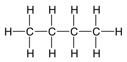
\includegraphics{desarrollada}
		\end{figure}
		\item \textbf{Fórmula Desarrollada} Se representan básicamente los enlaces del esqueleto carbonado y otros importantes, dejando sin desarrollar los de elementos menores (Hidrógenos). Es, con diferencia, la más utilizada en Química Orgánica:
			\begin{figure}[h!]
			\centering
			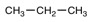
\includegraphics{semides}
		\end{figure}
		Existen también otros tipos de fórmulas que son derivadas de ésta última y que aumentan la esquematicidad de las mismas. Son las llamadas Fórmulas de Línea-Ángulo, donde se representan los enlaces por líneas y los carbonos por ángulos. También es frecuente esquematizar los sustituyentes mediante letras:
		\begin{figure}[h!]
			\centering
			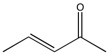
\includegraphics{lineangul}
			\caption{Representación de la \emph{3-penten-2-ona} según la forma línea-ángulo}
		\end{figure}  
\end{itemize}

\section{Número de Carbonos}
La parte más esencial de la nomenclatura orgánica, y que es común a todas las familias de compuestos, es el indicar el número de carbonos presentes en la molécula. Tal es así que, de forma general, se utilizarán una serie de prefijos en griego para denotar el número de carbonos en la molécula:
\begin{table}[h!]
	\centering
	\begin{tabular}{c|c||c|c}
		\textbf{Nº de Carbonos}&\textbf{Prefijos}&\textbf{Nº de Carbonos}&\textbf{Prefijos}\\ \hline
		Met-&1&Hex-&6\\
		Et-&2&Hept-&7\\
		Prop-&3&Oct-&8\\
		But-&4&Non-&9\\
		Pent-&5&Dec-&10\\ \hline
	\end{tabular}
\caption{Prefijos que indican Número de Carbonos}
\end{table}

\section{Hidrocarburos}
Los hidrocarburos son los compuestos orgánicos más sencillos que existen en la naturaleza. Están formados exclusivamente por Carbono e Hidrógeno, pudiendo estar unidos entre si mediante enlaces simples, dobles o triples.
\subsection{Hidrocarburos Saturados: Alcanos o Parafinas}
Son hidrocarburos simples formados por un esqueleto carbonado unido por enlaces simples. También se conocen como Hidrocarburos Saturados. Tienen como fórmula general $C_nH_{2n+2}$. El nombre de los mismos se construye añadiendo a los prefijos que indican el número de Carbonos la terminación \emph{-ano}.

\begin{figure}[h!]
	\centering
	\subfloat[Butano]{
	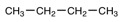
\includegraphics{butano}}
	\hspace{1cm}
	\subfloat[Hexano]{
	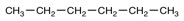
\includegraphics{hexano}}
\end{figure}
Para formular los alcanos (y cualquier compuesto orgánico por extensión) se siguen los siguientes pasos:\\

\begin{itemize}
	\item Se dibuja el esqueleto carbonado dibujando los enlaces C-C con el número de carbonos que indica el nombre de la molécula:
	\begin{center}
		C-C-C-C
	\end{center}
	\item Se completan con hidrógenos los carbonos de forma que llenemos sus cuatro valencias (es decir, nos aseguramos que cada carbono tenga 4 sustituyentes, ya sean hidrógenos, carbonos u otros elementos)
	\begin{figure}[h!]
		\centering
		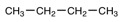
\includegraphics{butano}
	\end{figure}
	
\end{itemize}
\section{Cicloalcanos}
Son Hidrocarburos cuya cadena se encuentra cerrada sobre si misma, formando estructuras geométricas sencillas (triángulos, cuadrados, pentágonos, hexágonos….)
Aunque se pueden utilizar para representarlos la Fórmula Semidesarrollada, es mas usual hacerlo utilizando la Fórmula de Línea-Ángulo. Se nombran de igual manera que los alcanos de cadena abierta pero anteponiendo el prefijo \emph{Ciclo-}.
\begin{figure}[h!]
	\centering
	\subfloat[Ciclopropano]{
		
\includegraphics{ciclopropano}}
	\hspace{2cm}
	\subfloat[Ciclopentano]{
		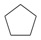
\includegraphics{ciclopentano}}
	\hspace{2cm}
	\subfloat[Ciclohexano]{
	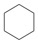
\includegraphics{ciclohexano}}
\end{figure}

\section{Alcanos Ramificados}
Son Alcanos Ramificados aquellos que poseen cadenas secundarias unidas a una cadena que consideramos primaria o principal. La cadena principal se nombra de igual modo que los alcanos y las cadenas secundarias utilizando el prefijo que indica el número de carbonos y la terminación -il. Las ramificaciones solo pueden estar en los carbonos mediales de la molécula, nunca terminales. Hay que recordar que las Fórmulas Orgánicas son representaciones bidimensionales de los compuestos, por lo que las fórmulas orgánicas tal y como las entendemos son una representación estática de un sistema dinámico y complejo, por lo que:

\begin{figure}[h!]
	\centering
	\subfloat[Metilpropano]{
		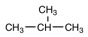
\includegraphics{metilpropano}}
	\hspace{1cm}
	\subfloat[Butano]{
		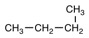
\includegraphics{butano2}}
\end{figure}

Cuando la ramificación pueda estar soportada en mas de un carbono distinto en la cadena principal, se nombra su posición usando números localizadores. Como norma general, entre número y letra se colocará un guión y entre número y número se colocarán comas.

\begin{figure}[h!]
	\centering
	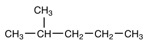
\includegraphics{metilpentano}
	\captionsetup{labelformat=empty}
	\caption{2-metilpentano}
\end{figure}

Los alcanos ramificados presentan tal complejidad a la hora de nombrarlos que es preciso  seguir una serie de normas o reglas establecidas por la IUPAC para la correcta confección de su nombre y su fórmula. Tales reglas son las siguientes:\\

\begin{enumerate}
	
	\item Se toma como cadena principal de la molécula la de mayor número de carbonos. Si hubiese dos cadenas con igual número de carbonos, entonces se tomará como principal la que contenga mayor número de ramificaciones o cadenas secundarias.
	\begin{figure}[h!]
		\centering
		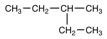
\includegraphics{3metilpentano}
		\captionsetup{labelformat=empty}
		\caption{3-metilpentano (en lugar de 2-etilbutano)}
	\end{figure}
	\item e numera la cadena principal de un extremo a otro de forma que los números localizadores de las cadenas secundarias sean los mas bajos posible
	\begin{figure}[h!]
		\centering
		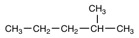
\includegraphics{2metilpentano}
		\captionsetup{labelformat=empty}
		\caption{2-metilpentano (en lugar de 4-metilbutano)}
	\end{figure}
	\item Si hubiese más de una cadena secundaria con el mismo número de átomos de carbono, se antepondrán al nombre los  prefijos de cantidad di-, tri-, tetra-,…
	\begin{figure}[h!]
		\centering
		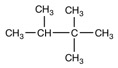
\includegraphics{trimetilbutano}
		\captionsetup{labelformat=empty}
		\caption{2,2,3-trimetilbutano}
	\end{figure}
	\item En caso de que hubiese distintas ramificaciones con distinto número de átomos de carbono, estas se ordenarán siguiendo riguroso orden alfabético. Para ello no se tendrán en cuenta los prefijos multiplicadores si los hubiera.
	\begin{figure}[h!]
		\centering
		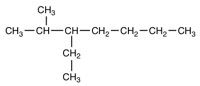
\includegraphics{metiletilheptano}
		\captionsetup{labelformat=empty}
		\caption{2-metil-3-etilheptano}
	\end{figure}
	\item Si en la molécula hubiera una ramificación que tuviera a su vez otra ramificación, estas se nombrarán entre paréntesis sabiendo que se tomará como carbono uno el más próximo a la cadena principal.
	 \begin{figure}[h!]
	 	\centering
	 	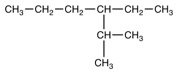
\includegraphics{metiletilhexano}
	 	\captionsetup{labelformat=empty}
	 	\caption{3-(1-metiletil)hexano}
	 \end{figure}
 \setcounter{nx}{\value{enumi}}
\end{enumerate}

\subsection{Hidrocarburos Insaturados (I): Alquenos u Olefinas}

Los Alquenos son hidrocarburos en donde al menos dos de sus carbonos están unidos entre si mediante un enlace doble. Se nombran utilizando los prefijos que indican el número de carbonos en la cadena principal seguido de la terminación \emph{-eno}\\
\begin{figure}[h!]
	\centering
	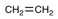
\includegraphics{eteno}
	\captionsetup{labelformat=empty}
	\caption{Eteno (también llamado comúnmente \emph{Etileno})}
\end{figure}

\begin{itemize}

\item Para cadenas mayores de tres átomos de carbono, es imprescindible localizar la posición del doble enlace en la cadena principal:
\begin{figure}[h!]
	\centering
	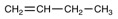
\includegraphics{1buteno}
	\captionsetup{labelformat=empty}
	\caption{1-buteno}
\end{figure}

\item Si en la cadena principal existiese mas de un doble enlace (polieno), estos se nombrarán anteponiendo los prefijos de cantidad a la terminación -eno:

\begin{figure}[h!]
	\centering
	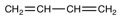
\includegraphics{13butadieno}
	\captionsetup{labelformat=empty}
	\caption{1,3-butadieno}
	\end{figure}
\end{itemize}

\subsection{Hidrocrburos Insaturados (II): Alquinos o Acetilenos}

Los Alquinos son hidrocarburos en donde al menos dos de sus carbonos están unidos entre si mediante un enlace triple. Se nombran utilizando los prefijos que indican el número de carbonos en la cadena principal seguido de la terminación \emph{-ino}.
\begin{itemize}
	
\begin{figure}[h!]
	\centering
	
\includegraphics{etino}
	\captionsetup{labelformat=empty}
	\caption{Etino (también llamado comúnmente \emph{Acetileno})}
\end{figure}
	\item Para cadenas mayores de tres átomos de carbono, es imprescindible localizar la posición del triple enlace en la cadena principal:

\begin{figure}[h!]
	\centering
	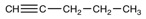
\includegraphics{1pentino}
	\captionsetup{labelformat=empty}
	\caption{1-pentino}
\end{figure}

	\item Si en la cadena principal existiese mas de un triple enlace, estos se nombrarán anteponiendo los prefijos de cantidad a la terminación \emph{-ino}:

\begin{figure}[h!]
	\centering
	
\includegraphics{14pentadiino}
	\captionsetup{labelformat=empty}
	\caption{1,4-pentadiino}
\end{figure}
\end{itemize}
\subsection{Hidrocarburos Insaturados Ramificados}

La introducción tanto de ramificaciones como de insaturaciones en los hidrocarburos hace que el número de compuestos orgánicos formados solamente por Carbono e Hidrógeno crezca de manera exponencial. Es necesario, por tanto, introducir nuevas reglas que se añadan o incluso modifiquen las existentes:\\

\begin{enumerate}
	\setcounter{enumi}{\value{nx}}
	\item La cadena principal será aquella que contenga mayor número de insaturaciones (dobles y triples enlaces). En el caso de que existan dos posibilidades que tengan igual numero de insaturaciones, se cogerá la mas larga. Y a igualdad de átomos de carbono, se escogerá la que contenga más número de dobles enlaces.\\
	
	\item Se numera la cadena principal de un extremo a otro de forma que los números localizadores de las insaturaciones sean lo mas bajos posibles. Si hay coincidencia, se comenzará por el extremo que le asigne números localizadores mas bajos a los dobles enlaces. A la hora de nombrarlos, los triples enlaces se nombran en último lugar.
	\begin{figure}[h!]
		\centering
		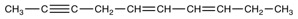
\includegraphics{octendiino}
		\captionsetup{labelformat=empty}
		\caption{3-octen-1,7-diino}
	\end{figure}
	\item Las ramificaciones no tienen prioridad con respecto a las insaturaciones, por lo que se nombran al principio y de acuerdo a las Reglas 3 y 4.
	\begin{figure}[h!]
		\centering
		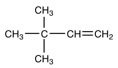
\includegraphics{dimetilbuteno}
		\captionsetup{labelformat=empty}
		\caption{3,3-dimetil-1-buteno}
	\end{figure}
	\item Las insaturaciones que recaigan sobre cadenas secundarias se nombrarán igualmente entre paréntesis y teniendo en cuenta que el carbono uno será el más próximo a la cadena principal.
	\begin{figure}[h!]
		\centering
		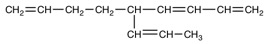
\includegraphics{putada}
		\captionsetup{labelformat=empty}
		\caption{5-(1-propenil)-1,3,8-octatrieno}
	\end{figure}
\end{enumerate}
Cuando tengamos dobles y triples enlaces en la misma molécula, generalmente el prefijo que indica el número de carbonos recae sobre el sufijo del doble enlace:\\

\begin{figure}[h!]
	\centering
	
\includegraphics{heptadienino}
	\captionsetup{labelformat=empty}
	\caption{3,5-heptadien-1-ino}
\end{figure}
\subsection{Hidrocarburos Halogenados}
Los Hidrocarburos halogenados, también llamados Haloalcanos o Haluros de Alquilo provienen de sustituir los hidrógenos de un Hidrocarburo (ya sea saturado o insaturado) por halógenos. Dichos halógenos han de ser localizados mediante sus correspondientes números localizadores, siempre que sea necesario.

\begin{figure}[h!]
	\centering
	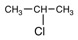
\includegraphics{cloropropano}
	\captionsetup{labelformat=empty}
	\caption{2-Cloropropano}
\end{figure}


%------------------------------------------------
% PART 2

\part{Herramientas Químicas}
%------------------------------------------------
% CHAPTER 3


\chapter{Química Cuantitativa}

\section{Introducción}
Se define la Química (del egipcio \emph{Keme}, “tierra”) como la ciencia que estudia la estructura, propiedades, composición y transformación de la materia. La química moderna se desarrolló a partir de la alquimia, una práctica protocientífica de carácter filosófico, que combinaba elementos de la química, la metalurgia, la física, la medicina, la biología, entre otras ciencias y artes. Esta fase termina al ocurrir la llamada,Revolución de la Química, basada en la Ley de conservación de la Masa y la teoría de la combustión por oxígeno postuladas por el científico francés, Antoine L. Lavoisier. \\
La Química a veces es definida como La Ciencia Central a causa de su rol de conexión y articulación entre las ciencias físicas, de las cuales forma parte, junto con las ciencias de la vida, y algunas ciencias aplicadas como la medicina o la ingeniería.

\section{Leyes Ponerales}

Las leyes ponderales de la Química son un conjunto de leyes de carácter empírico desarrolladas entre 1789 y 1803 por los primeros químicos que trataban de encontrar relaciones entre las masas de los compuestos químicos que intervenían en una reacción química. Posteriormente fueron generalizadas y superadas con la aparición de la teoría atómica y el concepto de mol.

\subsection{Ley de la Conservación de la Masa (Ley de Lavoisier)}

\textbf{Antonie-Laurent de Lavoisier (1743-1794)}, fue el primer químico que realizó cuidadosamente mediciones con la balanza, obteniendo una explicación correcta de las reacciones en las que metales como mercurio o cobre eran calentados en presencia de aire. En 1789, Lavoisier generalizó sus resultados a todas las reacciones químicas enunciando la llamada \emph{Ley de conservación de la masa}:\\

\begin{law}[Ley de Lavoisier]
En una reacción química, la masa total de las substancias que reaccionan (reactivos) es igual a la masa total de las substancias formadas (productos)
\begin{align}
\sum_{i = 1}^{N}(m_i)_{reactivos} = \sum_{i = 1}^{N}(m_i)_{productos}
\end{align}
\end{law}
\begin{figure}[h!]
	\centering
	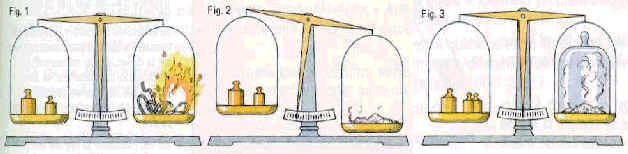
\includegraphics[width=0.8\textwidth]{lavoisier}
	\caption{Representación gráfica de las experiencias de Lavoisier}
\end{figure}

\subsection{Ley de las Proporciones Definidas (Ley de Proust)}

Si en condiciones cuidadosamente controladas, hacemos reaccionar por ejemplo, 10 g de cloro con 10 g de sodio, podrá probarse que los 10 g de cloro no reaccionan con todo el sodio, sino solo con una porción de él (6,484 g exactamente) quedándose el exceso sin reaccionar. Según la experiencia, el cloro y el sodio han reaccionado en la proporción en peso:\\

\begin{center}
	$\frac{m_{Na}}{m_{Cl}}=\frac{6,484}{10}$
\end{center}

\begin{law}[Ley de Proust]
	Cuando dos o más elementos se combinan para formar un determinado compuesto lo hacen en una relación en peso constante independientemente del proceso seguido para formarlo.
\end{law}

Esta ley fue enunciada por \emph{Louis Proust} en 1799, y atacada por \emph{C. L. Berthollet}, quién creía que la composición de un compuesto variaba según el método por el que se había preparado.\\

Modernamente se conocen compuestos sólidos que no cumplen la ley de las proporciones definidas (óxidos y sulfuras de elementos de transición), y se les llama compuestos no estequiométricos o \emph{Compuestos Berthóllidos}.\\

Podemos decir por tanto que:

\begin{center}
		$\frac{m_{Na}}{m_{Cl}}=\frac{6,484}{10}=\frac{12,968}{20}=\frac{4,934}{7,61}=cte$
\end{center}

Cada muestra de sal común descompuesta nos arrojará invariablemente un 39,34 \% de sodio y un 60,66 \% de cloro (relación 6,484/10)

\subsection{Ley de las Proporciones Múltiples (Ley de Dalton)}

La ley anterior no excluye la posibilidad de que dos sustancias puedan formar compuestos diferentes si varían las condiciones experimentales. De hecho, esto es lo que sucede, por ejemplo, con el oxígeno y el hierro o el cobre o el carbono, que dependiendo de las condiciones de la experiencia se originan óxidos diferentes. Para cada proceso individual, se cumple, por supuesto la ley de Proust, sin embargo, cabe hablar de otra más general que incluye estos casos. Veamos un ejemplo:\\

Al hacer reaccionar un gramo de oxígeno con cobre, la cantidad de éste consumida es exactamente 3,971 g:

\begin{center}
	$Oxígeno (1 gr) + Cobre  (3,971 gr) \rightarrow Óxido de Cobre
	$ 
\end{center}

Pero en condiciones experimentales diferentes, un gramo de oxígeno puede reaccionar con 7,942 g de cobre para dar lugar a otro compuesto diferente:

\begin{center}
	$Oxígeno (1 gr) + Cobre (7,942 gr) \rightarrow Óxido de Cobre’ $
\end{center}

Si dividimos los gramos de cobre que en ambos casos se combinaron con la misma cantidad (un gramo) de oxígeno, veremos que resulta una relación muy sencilla:

\begin{center}
	$\frac{3,971}{7,942}=\frac{1}{2}$
\end{center}

Lo anterior es un ejemplo de la Ley de las Proporciones Múltiples enunciada en 1803 por \emph{J. Dalton}:\\

\begin{law}[Ley de Dalton de las Proporciones Múltiple]
	Las cantidades de un mismo elemento que se combinan con una cantidad fija de otro para formar varios compuestos están en la relación de los números enteros sencillos
\end{law}

\subsection{Ley de las Proporciones Equivalentes (Ley de Richter)}

Fue enunciada por primera vez por \emph{J.B. Richter} en 1792. Es de importancia para la historia de la química y el desarrollo del concepto de mol y de fórmula química más que para la química actual. Esta ley permite establecer el peso equivalente o peso-equivalente-gramo, que es la cantidad de un elemento o compuesto que reaccionará con una cantidad fija de una sustancia de referencia.\\

\begin{law}[Ley de Richter]
	
	Las masas de dos elementos diferentes que se combinan con una misma cantidad de un tercer elemento, guardan la misma relación que las masas de aquellos elementos cuando se combinan entre sí.
\end{law}

\section{Teoría Atómica de Dalton}

El Químico inglés \emph{John Dalton (1766-1844)} fue uno de los primeros que reflexionó sobre estas leyes empíricas y otras leyes sobre el comportamiento de los gases, llegando a la conclusión de que los elementos químicos deberían estar constituidos por partículas pequeñísimas e indivisibles a las que denominó átomos. Mucho tiempo antes que él, el griego \emph{Demócrito de Abdera} había propuesto esta misma denominación para explicar los constituyentes íntimos de la materia. Dalton adoptó el mismo término. La llamada \textbf{Teoría Atómica de Dalton} establecía como puntos fundamentales que:

\begin{itemize}
	\item Los elementos químicos están formados por partículas (átomos) que son indivisibles e inalterables en todo proceso químico.\\
	\item Todos los átomos de un mismo elemento son exactamente ¡guales entre sí y distintos a los átomos de otro elemento diferente.\\
	\item Los compuestos se originan por la unión intensa de átomos distintos en una proporción constante.
\end{itemize}

Con estas ideas, Dalton podía explicar las leyes ponderales conocidas. En efecto, si los átomos son inalterables y una reacción química no es más que la reordenación de átomos, deberá haber el mismo número de estos átomos en todo el proceso, por lo que la masa debería permanecer inalterada.

\section{Leyes Volumétricas}

Son un conjunto de leyes de naturaleza empírica que relaciona los volúmenes de gases que intervienen en una reacción química.

\subsection{Ley de los Volúmenes de Combinación de Gay-Lussac}

El químico francés \emph{Joseph Louis Gay-Lussac} (1778-1850) estudió las reacciones en las que intervenían gases, realizando sus estudios en reacciones a Presión y Temperatura constantes. Tras estudiar distintos tipos de reacciones químicas (siempre en fase gaseosa) llegó a la conclusión que ocurría algo análogo a la la Ley de Proust cuando se medían los distintos volúmenes de las sustancias intervinientes en la reacción.\\



\begin{law}[Ley de los Volúmenes de Combinación de Gay-Lussac]
	Los volúmenes de las sustancias gaseosas que intervienen en una reacción química, medidos en las mismas condiciones de presión y temperatura, están en relación de números enteros sencillos.
\end{law}

\begin{center}
	\textbf{Cuando Dalton recibió esta información encontró algo que no cuadraba con su teoría de átomos indivisibles.}\\
\end{center}

Si la reacción de formación de agua se da en esas proporciones es evidente que la fórmula del agua no es $HO$, sino $H_2O$. Esto fue aceptado por Dalton (es una manera de determinar fórmulas) y supuso la corrección de la escala de masas atómicas relativas: el átomo de oxígeno tiene una masa igual a la de 16 átomos de hidrógeno.\\

Dalton aceptó que dos átomos de hidrógeno se combinaban con un átomo de oxígeno. Pero esta combinación debía producir una partícula (él la llamó átomo- compuesto) de agua, y por tanto, el volumen de agua obtenido debía ser un litro. Como Gay-Lussac informó de la obtención de dos litros de vapor de agua, Dalton supuso que tales medidas no podían ser correctas. Sin embargo, los datos obtenidos en el laboratorio eran claros: Gay-Lussac no estaba equivocado, un litro de oxígeno se combina con dos litros de hidrógeno y produce dos litros de vapor de agua. La solución vendría de otro químico genial: \textbf{Amadeo Avogadro}.

\subsection{Hipótesis de Avogadro}

En sus hipótesis Avogadro sugiere que las partículas de los gases son en realidad de dimensiones mucho menores que el volumen del recipiente que las contienen, de forma que estas no están en reposo como creía Dalton, sino están muy separadas en continuo movimiento. Sin esta condición no parecería lógico que moléculas grandes o pequeñas ocuparan el mismo volumen. Pronto se comprobó que las partículas de los gases elementales son moléculas diatómicas y la primera utilidad fue la determinación de fórmulas de compuestos y, por tanto, la determinación de las masas atómicas relativas correctas.\\

Según Avogadro:

\begin{itemize}
	\item Cada molécula de agua debe tener, como mínimo, un átomo de oxígeno. Si el volumen de agua que se obtiene es el doble que el de oxígeno, la molécula de oxígeno debe ser diatómica, para que cada molécula origine los átomos que permitan formar dos moléculas de agua.\\
	\item Como el volumen de agua es el mismo que el de hidrógeno, debe haber el mismo número de moléculas de cada uno.
\end{itemize}

\begin{law}[Hipótesis de Avogadro]
	En condiciones iguales de presión y temperatura, volúmenes iguales de gases diferentes tienen el mismo número de moléculas....
\end{law}

\section{Concepto de Mol}

Determinar la masa de un átomo o de una molécula es evidentemente imposible usando las balanzas, de ahí que los químicos hayan decidido definir una "nueva" unidad para medir la masa de átomos y moléculas. A esa unidad se la denomina unidad de masa atómica (uma) y ya que el hidrógeno se ha comprobado que es el elemento de menos masa es lógico definirlo como unidad, definirlo como uma.\\

Así en una primera aproximación diremos que la unidad de masa atómica es simplemente la masa de un átomo de hidrógeno. De modo que si decimos que, por ejemplo, el carbono tiene de masa atómica 12 urna, con ello estamos diciendo que un átomo de carbono pesa 12 veces más que un átomo de hidrógeno, o si decimos que la molécula de agua pesa 18 urna, decimos que una molécula de agua pesa 18 veces más que un átomo de hidrógeno, y así sucesivamente.\\

Lógicamente la masa de una molécula (masa molecular) se obtendrá por la suma de las masas atómicas de cada uno de los elementos que la forman. Esos datos de masas atómicas vienen recogidas en la tabla periódica. Con todo, en los laboratorios las balanzas no miden uma, sino gramos, de ahí que haga falta hallar una relación entre ambas escalas.\\


Mil moléculas (o átomos) de cualquier especie es aún un número muy pequeño para poder pesarse en la balanza, pero todo es cuestión de escoger un número muy grande de moléculas (o átomos) que podamos pesar. Lógicamente, 1000 átomos de carbono, por ejemplo, pesarían en uma $12\cdot 1000$. Si en lugar de elegir mil elegimos $10^{23}$ resulta que ese es un número ya muy muy grande. Si escogemos $6,02\cdot10^{23}$ átomos de carbono, éstos pesarán $12\cdot6,02\cdot10^23$ uma, pero curiosamente, al poner todos esos átomos sobre la balanza, "curiosamente" pesan 12 gramos.\\

\begin{definition}[Mol]
	El mol corresponde con la cantidad de materia que contiene $6.022\cdot10^{23}$ átomos o moléculas de una determinada sustancia
\end{definition}

Esa es la ventaja de elegir “ese número tan raro", que \textbf{la masa en gramos de la especie elegida coincide numéricamente con la masa en uma}. A ese “número tan raro” se le conoce con el nombre de \textbf{Número de Avogadro}:\\

\begin{center}
$N_A=6,02\cdot10^{23}$
\end{center}
Por todo lo anteriormente expuesto aquí, existe una manera de calcular la equivalencia entre gramos y moles de una substancia:

\begin{definition}[Definición de Mol]
	Se define el Mol como los gramos de una determinada sustancia dividida por su masa molecular:
	\begin{align}
		& n=\frac{gr}{M_m}
	\end{align}
\end{definition}

\begin{exercise}
	\textbf{Calcula los moles de moléculas de Ácido Sulfúrico contenidas en 100 gr de dicha substancia. Calcula también los moles y el número de átomos de oxígeno.}\\
	
	La masa molecular del ácido sulfúrico ($H_2SO_4$) es:
	$M_m = 2\cdot1 + 1\cdot32 + 4\cdot16 = 98 gr/mol$\\
	
	El número de moles de Ácido Sulfúrico por tanto, es:
	$n = \frac{100}{98} = $1,021 moles de $H_2SO_4$\\
	
	Y el número de moléculas: 
	$1,021\cdot6,02\cdot10^{23} = 6,14\cdot10^{23}$  moléculas de $H_2SO_4$\\
	
	Puesto que existen 4 átomos de oxígeno por molécula de ácido sulfúrico:\\
	
	1,021 moles de $H_2SO_4 \cdot 4 = 4,84$ moles de átomos de oxígeno
	
	$4 \cdot 6,14 \cdot10^{23}$  moléculas de $H_2SO_4 = 2,46 \cdot10^{24}$ átomos de oxígeno
	
\end{exercise}

\section{Concepto de Equivalente}

Se define \emph{Equivalente o Equivalente Gramo} a la masa de una substancia dada que:\\

\begin{itemize}
	\item Sustituye o reacciona con un mol de iones hidrógeno ($H^+$) en una reacción ácido-base.\\
	\item Sustituye o reacciona con un mol de electrones en una reacción redox.\\
\end{itemize}

El concepto de equivalente es de gran utilidad sobre todo en reacciones ácido-base y redox, puesto que en dichas reacciones las sustancias intervinientes lo hacen equivalente a equivalente, lo cual simplifica muchísimo los cálculos. Se puede calcular:\\

\begin{definition}[Equivalente]
	
	Se define Equivalente como los gramos de cierta sustancia divididos entre su Masa Equivalente
	
	\begin{align}
		& eq =\frac{gr}{M_{eq}}
	\end{align}
	
\end{definition}

Como podemos observar la similitud con la definición de Mol es evidente, como evidente es también la semejanza entre Masa Equivalente y masa Masa Molecular:\\

\begin{definition}[Masa Equivalente]

Se define Masa Equivalente de una sustancia en una reacción química dada como la Masa Molecular de dicha sustancia entre su valencia en dicha reacción química, entendiendo por valencia el número de Hidrógenos intercambiados en una reacción ácido-base o el número de electrones cedidos o absorbidos en una reacción Redox

\begin{align}
	& M_{eq} = \frac{M_{m}}{Val}
\end{align}

\end{definition}

\section{Modelo del Gas Ideal}

Un gas ideal es un modelo teórico que explica el comportamiento de los gases, simplificando su comportamiento y permitiendo su estudio teórico de manera sencilla. Dicho modelo se basa en las siguientes premisas:
\\

\begin{enumerate}
	\item El número de partículas constituyentes del gas es muy grande, como también lo son las distancias entre ellas en comparación con el recipiente que las contiene. Por tanto, podemos considerar las partículas como masas puntuales con un volumen despreciable\\
	\item Las partículas que forman el gas se encuentran en continuo movimiento, caótico y muy rápido.\\
	\item Las partículas chocan entre si elásticamente. También se producen choques elásticos con las paredes del recipiente, siendo la Presión del gas el resultado macroscópico de dicho movimiento.\\
	\item Se consideran despreciables las fuerzas entre partículas, salvo en el momento de los choques. Esto implica que los gases ideales no licúan.\\
	\item El gas es considerado puro, es decir, todas las moléculas son iguales.\\
\end{enumerate}

Solo los gases mas ligeros en condiciones de bajas presiones y temperaturas tienen un comportamiento que se aproxima al del gas ideal. Sin embargo, las conclusiones extraídas de dicho modelo resultan altamente valiosas a la hora de estudiar (y entender) el comportamiento de los gases reales.

\subsection{Ecuación de Estado de los Gases Ideales}

Se definen las \emph{Variables de Estado} de un sistema como aquellas que por si mismas son capaces de definir totalmente el estado de un sistema fisicoquímico. En el caso de los gases, estas variables de estado son tres, a saber, \textbf{Presión, Volumen y Temperatura}.\\

Para el caso de los Gases Ideales, existe una ecuación que relaciona de manera extremadamente sencilla y eficaz las tres variables de estado. A esta relación se le conoce como \textbf{Ecuación de Estado de los Gases Ideales}:

\begin{definition}[Ecuación de Estado de los gases Ideales]
	El producto de la Presión a la que está sometido un Gas Ideal por su Volumen es directamente proporcional a la temperatura de éste:
	
	\begin{align}
		& P\cdot V = n\cdot R \cdot T
	\end{align}
	
\end{definition}

Donde P se mide en atmósferas, V en litros, n en moles y T en Kelvin. A R se le conoce como constante de los gases ideales, y su valor es $R = 0,082 atm \cdot l/ mol\cdot K$. La Ley de los gases ideales es totalmente coherente con las leyes de Gay-Lussac y Boyle-Mariotte estudiadas en cursos anteriores.\\

Una de las características mas destacables de la Ecuación de los Gases Ideales es que es totalmente independiente de de la naturaleza del gas que estemos estudiando, lo cual hace de ella una herramienta prácticamente universal.\\

\begin{exercise}
	\textbf{Calcula el Volumen que ocupará un mol de Gas Ideal medido en Condiciones Normales.}\\
	
	En Química se definen las Condiciones Normales (C.N) a aquellas correspondientes a P = 1 atm y T = 273 K. Por tanto:\\
	
	$V = \frac{n \cdot R \cdot T}{V} = \frac{1 \cdot 0,082 \cdot 273}{1} = 22,4 l$
		
\end{exercise}

Según lo dicho anteriormente, la ecuación de los gases ideales no depende de la naturaleza del gas. Por tanto se puede concluir que:\\

\begin{definition}[Volumen de un Gas Ideal en CN]
	Un mol de cualquier gas ideal medido en Condiciones Normales ocupa un Volumen de 22,4 l
\end{definition}

\subsection{Mezcla de Gases: Ley de Dalton de las Presiones Parciales}

Puesto que es casi imposible encontrar reactivos que sean químicamente puros, por norma general los gases se encuentran formando mezclas, por lo que su estudio se hace mas difícil. Fue el científico ingles J. Dalton quien en 1801 resolvió el problema enunciando la \textbf{Ley de las Presiones Parciales}\\

\begin{definition}[Presión Parcial de un gas]
	Se define la Presión Parcial de un gas en una mezcla como aquella que tendría dicho gas si en el recipiente que contiene la mezcla estuviese el solo a las mismas condiciones de Temperatura 
\end{definition}

Por tanto podemos enunciar:

\begin{law}[Ley de Dalton de las Presiones Parciales]
	La presión de una mezcla de gases ideales que no reaccionan químicamente, es igual a la suma de las presiones parciales que ejercería cada uno de ellos si sólo uno ocupase todo el volumen de la mezcla:\\
	
		$P_T = \displaystyle\sum_{i=1}^{N}P_i$\\
		
		$P_i = X_i \cdot P_T$
		
\end{law}

Donde $P_T$ es la presión total, $P_i$ la presión parcial de gas en la mezcla y $X_i$ la fracción molar del gas en dicha mezcla.\\

Si estamos ante el caso de un gas ideal, la ecuación de estado también se puede aplicar a cada gas por separado:

\begin{center}
	$P_i = n_i \cdot R \cdot T$
\end{center}

\section{Análisis Elemental y Composición Centesimal}

Uno de los primeros problemas al que se enfrenta un químico cuando se encuentra ante un compuesto químico desconocido es hallar cual es su composición. Esto es de vital de importancia si nos encontramos ante un compuesto orgánico, en donde el primer paso será siempre el encontrar su formula molecular, como actuación previa para poder determinar su estructura. Así definimos composición centesimal como el porcentaje en masa de cada uno de los elementos que forman un compuesto en relación a la masa total.

\begin{exercise}
	\textbf{Indica la Fórmula Molecular de un compuesto químico que contiene 40 \% de C, 6,7 \% de H y 53,3 \% de O. Su masa molecular obtenida por espectrometría de masas es 60 gr/mol.}\\
	
	Dividimos cada uno de los porcentajes entre su masa atómica:\\
	
	$C: \frac{40}{12}=3,33$
	$H: \frac{6,7}{1}=6,7$ 
	$O: \frac{53,3}{16}=3,33$\\
	
	A continuación dividimos entre el número más bajo para establecer la proporción:\\
	
	$C: \frac{3,33}{3,33}=1$
	$H: \frac{6,7}{3,33} \simeq 2$ 
	$O: \frac{53,3}{16}=1$\\
	
	Por tanto la fórmula empírica del compuesto es $(CH_2O)_x$, cuya masa molecular es $M_{FE} = 12 + 2 \cdot 1 + 16 = 30$ gr/mol.\\
	
	Para calcular la formula molecular, dividimos la masa molecular del compuesto entre la masa molecular de la fórmula empírica:
	$x = \frac{60}{30}=2$\\
	
	Por lo que la fórmula molecular del compuesto será $(CH_2O)_2 = C_2H_4O_2$
	
\end{exercise}

\subsection{Análisis Elemental por Combustión}

El método clásico para realizar un análisis elemental se basa en el hecho de que cualquier hidrocarburo sometido a una combustión genera como productos $CO_2$ y $H_2O$:\\

\begin{center}
	$C_xH_yO_z + O_2 \rightarrow mCO_2 + nH_2O$
\end{center}

El aparato analizador consiste en en una cámara cerrada en donde se produce una combustión total del analito. El tren de gases producido se hace pasar por un montaje que incluye un primer recipiente en donde nos encontramos con un agente anhidro ($Mg(ClO_4)_2$ o $CaCl_2$) que atrapa todo el agua generada. Posteriormente se dispone un segundo recipiente que contiene una base fuerte (normalmente KOH) para atrapar todo el CO2 formado. La diferencia de peso de los recipientes antes de la combustión y después nos dará la cantidad de $CO_2$ y $H_2O$ formadas. Es, por tanto, un método de análisis gravimétrico. 

\begin{exercise}
	\textbf{Por combustión de 0,25 gr de una substancia orgánica compuesta por C, H y O, se obtienen 0,568 gr de $CO_2$ y 0,232 gr de $H_2O$. Calcula la fórmula empírica del compuesto.}\\
	
	El objetivo va a ser calcular el número de moles de átomos de C, H y O presentes en la muestra. En el caso de los dos primeros es directo:
	
	C: $\frac{0,568}{44}  = 0,0129 moles CO_2 \cdot 1 = 0,0129$ moles de C
	
	H: $\frac{0,232}{18} = 0,0128 moles de H_2O \cdot 2 = 0,0257$ moles de H\\
	
	En el caso del Oxígeno es un poco más complicado, pues la cantidad presente en $CO_2$ y $H_2O$ proviene tanto del compuesto problema como del $O_2$ del aire. Por tanto, sacamos los gr de C e H atómicos:\\
	
	C: $0,0129\cdot 12 = 0,1549$ gr de C
	
	H: $0,0257\cdot 1 = 0,0257$ gr de H\\
	
	Y aplicando la Ley de Lavoisier:
	
	$m_O$ = 0,25 -(0,1549 + 0,0257) = 0,0694 gr de O / 16 = 0,0044 moles de O\\
	
	Ahora dividimos entre el menor número de moles atómicos:\\
	
	C: $\frac{0,0118}{0,0043} = 3$
	
	H: $\frac{0,0257}{0,0043} = 6$
	
	O: $\frac{0,0043}{0,0043} = 1$\\
	
	Luego la fórmula empírica del compuesto es $C_3H_6O$
	
\end{exercise}

\section{Disoluciones}

Una disolución se define como una mezcla homogénea en la cual uno de los componentes (disolvente) se encuentra en mucha mayor proporción que el otro (soluto). Tanto disolvente como soluto pueden estar en cualquiera de los tres estados de agregación de la materia, dando lugar a infinidad de tipos distintos de disoluciones:\\

\begin{figure}[h!]
	\centering
	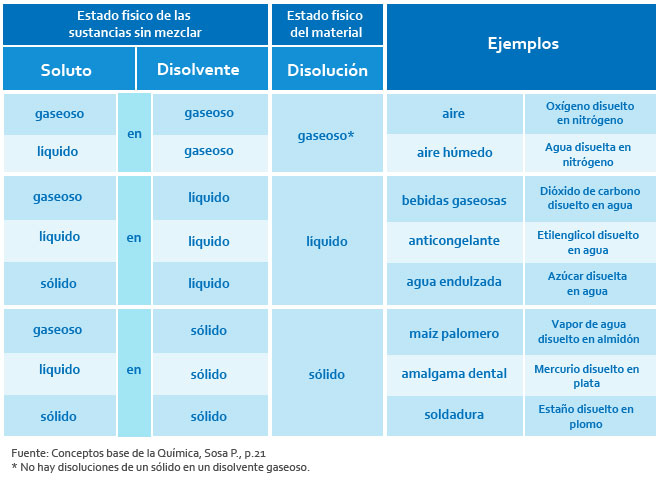
\includegraphics[width = 0.8\textwidth]{dis}
	\caption{Resumen de los distintos tipos de disoluciones}
\end{figure}  

El estudio de las disoluciones en química se hace de vital importancia debido a que la inmensa mayoría de reacciones químicas tienen lugar mediante disoluciones acuosas.

\subsection{Formas de Expresar la Concentración}

Existen varias formas matemáticas de expresar la concentración en una disolución:\\

\begin{definition}[Porcentaje en Masa]
	Se define como la masa de soluto entre la masa total de disolución:
	\begin{align}
		& \%(m/m)=\frac{m_{sol}}{m_{sol}+m_{dvte}}x100
	\end{align}
\end{definition}

\begin{definition}[Porcentaje en Volumen]
Se define como el volumen de soluto entre el volumen total de disolución:
	\begin{align}
	& \%(v/v)=\frac{v_{sol}}{v_{sol}+v_{dvte}}x100
	\end{align}
Se suele utilizar en el caso de disoluciones con solutos líquidos.
\end{definition}

\begin{definition}[Gramos por Litro]
	Se define como los gramos de soluto entre el volumen total en litros de la disolución:
	\begin{align}
		& gr/l =\frac{gr_{sol}}{V(l)_{dison}}
	\end{align}
\end{definition}

\begin{definition}[Molaridad]
	Se define como los moles de soluto entre el volumen total en litros de la disolución:
	\begin{align}
		& M =\frac{n_{sol}}{V(l)_{dison}}
	\end{align}
Es, con diferencia, la más utilizada de todas.
\end{definition}

\begin{definition}[Molalidad]
	Se define como los moles de soluto entre los kilogramos de disolvente:
	\begin{align}
		& m =\frac{n_{sol}}{m(Kgr)_{dvte}}
	\end{align}
\end{definition}

\begin{definition}[Normalidad]
	Se define como los equivalentes de soluto entre el volumen total en litros de la disolución:
	\begin{align}
		& N =\frac{eq_{sol}}{V(l)_{dison}}
	\end{align}
\end{definition}

Debido a su relación con la Molaridad, ambas magnitudes se pueden expresar: \textbf{$N = M\cdot val$}

\begin{definition}[Fracción Molar de Soluto]
Se define como la proporción molar de soluto en la disolución expresada en tanto por uno:
	\begin{align}
		& X_s=\frac{n_{sol}}{n_{sol}+n_{dvte}}
	\end{align}
\end{definition}

\begin{definition}[Fracción Molar de Disolvente]
	Se define como la proporción molar de disolvente en la disolución expresada en tanto por uno:
	\begin{align}
		& X_d=\frac{n_{dvte}}{n_{sol}+n_{dvte}}
	\end{align}
\end{definition}

En ambas fracciones molares se cumple que: \textbf{$X_s + X_d = 1$}\\

En los cálculos con disoluciones se suele utilizar de manera habitual la densidad. Por tanto, es útil recordar que la densidad relaciona la masa de la disolución con el volumen de dicha disolución:\\

\begin{center}
	$d=\frac{m_{dison}}{V_{dison}}$
\end{center}

\begin{exercise}
	\textbf{Un ácido sulfúrico comercial tiene una etiqueta que indica 95 \%(m/m) y  d = 1,83 $gr/cm^3$. Calcula su molaridad, molalidad, normalidad, gramos litro y fracciones molares de soluto y disolvente.}\\
	
	Del dato de porcentaje podemos deducir que en 100 gr de disolución hay 95 gr de soluto puro y por tanto 5 gr de disolvente puro. Por tanto podemos utilizar estos datos para obtener el volumen de la  disolución:\\
	
	$V_{dison}=\frac{M_{dison}}{d}=\frac{100}{1,83}=$ 54,64 ml\\
	
	Por otro lado, y sabiendo que la Masa molecular del ácido sulfúrico es 98 gr/mol, podemos calcular algunas magnitudes:\\
	
	$M = \frac{\frac{95}{98}}{0,05464}=$ 17,74 M\\
	
	$gr/l = \frac{95}{0,05464}=$ 1738,6 gr/l\\
	
	$m = \frac{\frac{95}{98}}{0,005}=$ 19,38 mol/Kg\\
	
	Puesto que el $H_2SO_4$ contiene dos hidrógenos, su valencia es dos y, por tanto, su Normalidad:\\
	
	$N=M\cdot val=17,74\cdot 2=$ 35,48 N\\
	
	Y sus fracciones molares de soluto y disolvente:\\
	
	$X_s = \frac{\frac{95}{98}}{\frac{95}{98}+\frac{5}{18}}= 0,78$\\
	
	$X_d=1-X_s=0,22$
\end{exercise}

\subsection{Diluciones}

Se puede definir una dilución en una disolución acuosa como el proceso de añadir agua pura a una alícuota de una disolución concentrada para que su concentración sea menor. En un laboratorio químico es una tarea bastante común puesto que muchos compuestos que se utilizan de manera muy habitual (cómo algunos ácidos inorgánicos) suelen venir en forma de disolución muy concentrada. El cálculo de diluciones se basa en el hecho de que el número de moles de soluto presentes en la alícuota de la disolución concentrada es el mismo que en la disolución diluida, pues la variación de la concentración de la disolución se debe al aumento del volumen de la misma.\\

\begin{center}
	$n_{conc}=n_{dil}$
\end{center}

Y sustituyendo en la definición de Molaridad:\\

\begin{center}
	$V_{conc}\cdot M_{conc}=V_{dil}\cdot M_{dil}$
\end{center}

\begin{exercise}
	\textbf{Queremos preparar 250 ml de una disolución 0,5 M de Ácido Sulfúrico a partir de una disolución comercial de 95 \% (m/m) y d = 1,83 $gr/cm^3$. Calcula el volumen necesario que debemos tomar de la disolución comercial para obtener la dilución.}\\
	
	Lo primero que debemos de hacer es expresar la concentración del ácido comercial en molaridad (pues lo más común es que las etiquetas nos indiquen densidad y porcentaje en masa). Omitiremos los cálculos, puesto que son los mismos que en el ejercicio anterior. Por tanto, una disolución 95 \%(m/m) y de densidad 1,83 $gr/cm^3$ es equivalente a una disolución 17,74 M. Por ello, y teniendo en cuenta que el número de moles de soluto no varía en la disolución comercial:\\
	
	$V_{conc}\cdot M_{conc}=V_{dil}\cdot M_{dil}$\\
	
	Como nos piden el volumen de la concentrada:\\
	
	$V_{conc}=\frac{V_{dil}\cdot M_{dil}}{M_{conc}}= \frac{250\cdot 0,5}{17,74}=$ 7 ml\\
		
	Luego si cogemos una alícuota de 7 ml de la disolución comercial y completamos en un matraz aforado hasta los 250 ml, obtendremos una disolución 0,5 M.
	
\end{exercise}

\section{Estequiometría}

Se puede definir Estequiometría como el cálculo de las relaciones cuantitativas entre los reactivos y los productos de una reacción química. Estas relaciones se pueden deducir en base a la teoría atómica, aunque históricamente se desarrollaron siguiendo principios y leyes empíricas.Constituye en si misma uno de los pilares básicos del trabajo en el laboratorio, por lo que se hace imprescindible su estudio en esta asignatura.

\subsection{Ajuste de Reacciones Químicas}

Una reacción química se puede definir como un cambio en la ordenación de los átomos entre los reactivos y los productos para dar compuestos químicos totalmente distinto. Puesto que ningún proceso químico puede violar la Ley de Lavoisier de Conservación de la Masa, se hace necesario antes de entrar en cualquier consideración de carácter cuantitativo asegurarse que el numero total de átomos presentes tanto en reactivos como en productos sean iguales (ya que la materia se conserva y ningún átomo puede aparecer o desaparecer de la nada) A este proceso se le conoce como \textbf{Ajuste de una Reacción Química}.\\

Por ejemplo, para la reacción de formación del agua:\\

\begin{center}
	$H_2 + O_2 \longrightarrow H_2O$
\end{center}

Si observamos bien nos daremos cuenta que en el balance global de átomos, a la derecha solo hay un átomo de oxígeno y a la derecha dos. La forma de solventar esto sería multiplicar por dos el agua. Pero si multiplicamos el agua se nos modifica tanto el número de oxígenos como el número de hidrógenos, por lo que habría que multiplicar por dos también el hidrógeno molecular, quedándose totalmente ajustada la reacción.\\

\begin{center}
	$2H_2 + O_2 \longrightarrow 2H_2O$
\end{center}

Por lo tanto para que se cumpla la Ley de Conservación de la Masa tiene que ocurrir que:\\

\begin{center}
\textbf{2 moléculas de Hidrógeno reaccionan con una molécula de Oxígeno para dar 2 moléculas de agua}
\end{center}

La escala atómica es demasiado pequeña para manipularse en un laboratorio. Pero como la reacción es proporcional también se puede cumplir tomando como referencia el mol. Así pues:\\

\begin{center}
\textbf{2 moles de Hidrógeno reaccionan con un mol de Oxígeno para dar 2 moles de agua}
\end{center}

\subsection{Estequimetría con un Reactivo en Exceso}

Sería el caso mas simple de todos, aquel en el que la cantidad de un reactivo es lo suficientemente mayor como para que no haya que tenerlo en cuenta a la hora de hacer los cálculos.\\

\begin{exercise}
	\textbf{Se hacen reaccionar 15 gr de Hidrógeno con exceso de oxígeno. Calcula la cantidad de agua formada.}\\
	
	Escribimos la reacción química:\\
	
	\begin{center}
		$2H_2 + O_2 \longrightarrow 2H_2O$
	\end{center}
	
	Calculamos después los moles de hidrógeno que se hacen reaccionar:\\
	
	n = 15 / 2 = 7,5 moles de Hidrógeno\\
	
	Y ahora planteamos un regla de tres con la proporción que nos indica la reacción:\\
	\begin{equation*}
	
	2 moles de $H_2$ \hline 1 mol $O_2$\\
	
	7,5 moles de $H_2$ \hline x mol $O_2$
	\right |
	\quad\text{x = 3,75 moles de $O_2$}
	\end{equation*}
\end{exercise}
%------------------------------------------------

% CHAPTER 4
\chapter{Termodinámica Química}

\section{Introducción}

La \textbf{Termodinámica} es la parte de la Física que se ocupa del estudio de las relaciones que se establecen entre el calor y el resto de las formas de energía. Entre otras cuestiones la termodinámica se ocupa de analizar los efectos que producen los cambios de magnitudes tales como la temperatura, la densidad, la presión, la masa, el volumen, en los sistemas y a un nivel macroscópico. La base sobre la cual se ciernen todos los estudios de la termodinámica es la circulación de la energía y como ésta es capaz de infundir movimiento. Vale destacar que justamente esta cuestión fue la que promovió el desarrollo de esta ciencia, ya que su origen se debió a la necesidad de aumentar la eficiencia de las primeras máquinas de vapor.\\

Los primeros estudios termodinámicos se deben al ingeniero francés \emph{Nicolas Sadi Carnot (1796-1832)}, quien en 1824 publico un libro titulado \emph{Reflexiones sobre la Fuerza Motriz del Fuego}, donde abordaba la eficiencia de las máquinas de vapor que se utilizaban en la época y los máximos rendimientos que se podían alcanzar con una máquina térmica ideal a la cual se llamó \textbf{Maquina de Carnot}.\\

Las conclusiones obtenidas por Carnot y sus sucesores fueron tan generales y simples que la termodinámica se ha establecido como una disciplina general que se ocupa de describir cómo los sistemas responden a los cambios que se producen en su entorno, pudiéndose aplicar a una infinidad de situaciones tanto de la ciencia como de la ingeniería, como pueden ser: motores, reacciones químicas, transiciones de fase, fenómenos de transporte, agujeros negros… entre otras. 

\section{Termoquímica}

Se define \textbf{Termoquímica} como la parte de la Química que estudia las transferencias energéticas en el transcurso de una reacción química. Dicha energía se manifiesta mayoritariamente en forma de calor, por lo que se puede resumir la termoquímica como la parte de la química que estudia el intercambio calorífico que tiene lugar en una reacción química. Como dicho calor tiene que ver con el contenido de energético de los compuestos químicos intervinientes en el proceso, y teniendo en cuenta que todo sistema químico tiende al estado de mínima energía, la termoquímica se encarga también del estudio de la espontaneidad de las reacciones químicas. 

\section{Sistema Termodinámico}

Se define \textbf{Sistema Termodinámico} como una porción del universo físico que se aísla para su estudio. A la porción del universo físico que se encuentra en contacto con nuestro sistema se le denomina \textbf{Entorno}. Los sistemas termodinámicos se clasifican según el grado de aislamiento que presentan con su entorno. Aplicando este criterio pueden darse tres clases de sistemas:\\

\begin{itemize}
	\item \textbf{Sistema aislado:} Es aquel que no intercambia ni materia ni energía con su entorno, es decir se encuentra en equilibrio termodinámico. Un ejemplo de esta clase podría ser un gas encerrado en un recipiente de paredes rígidas lo suficientemente gruesas (paredes adiabáticas) como para considerar que los intercambios de energía calorífica sean despreciables y que tampoco puede intercambiar energía en forma de trabajo.\\
	
	\item \textbf{Sistema Cerrado:} Es aquel que puede intercambiar energía pero no materia con el exterior. Multitud de sistemas se pueden englobar en esta clase. El mismo planeta Tierra puede considerarse un sistema cerrado. Una lata de sardinas también podría estar incluida en esta clasificación.\\
	
	\item \textbf{Sistema Abierto:} En esta clase se incluyen la mayoría de sistemas que pueden observarse en la vida cotidiana. Por ejemplo, un vehículo motorizado es un sistema abierto, ya que intercambia materia con el exterior cuando es cargado, o su conductor se introduce en su interior para conducirlo, o es provisto de combustible al repostarse, o se consideran los gases que emite por su tubo de escape pero, además, intercambia energía con el entorno. Solo hay que comprobar el calor que desprende el motor y sus inmediaciones o el trabajo que puede efectuar acarreando carga.\\
	
\end{itemize}
	
	Puesto que la gran mayoría de reacciones químicas tienen lugar en disolución, es decir, en un vaso de precipitados, los sistemas químicos se consideran en su mayor parte como \emph{sistemas abiertos}.
	
\section{Variables de Estado}

Una vez determinados los límites de un sistema termodinámico objeto de estudio o investigación, se procede a determinar y cuantificar su estado. En Termodinámica, se denominan \emph{Variables de Estado} a aquellas variables que caracterizan un sistema. Dichas variables son variables macroscópicas, perfectamente medibles en un laboratorio por métodos simples y que caracterizan un estado microscópico concreto. Por ejemplo, en un sistema termodinámico formado por un gas, las variables de estado son la \emph{Presión, Volumen y Temperatura}.\\

Las variables de estado tienen una característica fundamental e importantísima en un proceso: \textbf{Solo dependen de los estados inicial y final del sistema, nunca del proceso seguido}. Esto es de una importancia vital a la hora de estudiar un sistema químico, pues durante una reacción química las variables de estado van a depender exclusivamente de los estados inicial y final, esto es, reactivos y productos, simplificando enormemente el tratamiento teórico de los mismos.


%------------------------------------------------

\section{Citation}\index{Citation}

This statement requires citation \cite{book_key}; this one is more specific \cite[122]{article_key}.

%------------------------------------------------

\section{Lists}\index{Lists}

Lists are useful to present information in a concise and/or ordered way\footnote{Footnote example...}.

\subsection{Numbered List}\index{Lists!Numbered List}

\begin{enumerate}
\item The first item
\item The second item
\item The third item
\end{enumerate}

\subsection{Bullet Points}\index{Lists!Bullet Points}

\begin{itemize}
\item The first item
\item The second item
\item The third item
\end{itemize}

\subsection{Descriptions and Definitions}\index{Lists!Descriptions and Definitions}

\begin{description}
\item[Name] Description
\item[Word] Definition
\item[Comment] Elaboration
\end{description}

%----------------------------------------------------------------------------------------
%	CHAPTER 2
%----------------------------------------------------------------------------------------

\chapter{In-text Elements}

\section{Theorems}\index{Theorems}

This is an example of theorems.

\subsection{Several equations}\index{Theorems!Several Equations}
This is a theorem consisting of several equations.

\begin{theorem}[Name of the theorem]
In $E=\mathbb{R}^n$ all norms are equivalent. It has the properties:
\begin{align}
& \big| ||\mathbf{x}|| - ||\mathbf{y}|| \big|\leq || \mathbf{x}- \mathbf{y}||\\
&  ||\sum_{i=1}^n\mathbf{x}_i||\leq \sum_{i=1}^n||\mathbf{x}_i||\quad\text{where $n$ is a finite integer}
\end{align}
\end{theorem}

\subsection{Single Line}\index{Theorems!Single Line}
This is a theorem consisting of just one line.

\begin{theorem}
A set $\mathcal{D}(G)$ in dense in $L^2(G)$, $|\cdot|_0$. 
\end{theorem}

%------------------------------------------------

\section{Definitions}\index{Definitions}

This is an example of a definition. A definition could be mathematical or it could define a concept.

\begin{definition}[Definition name]
Given a vector space $E$, a norm on $E$ is an application, denoted $||\cdot||$, $E$ in $\mathbb{R}^+=[0,+\infty[$ such that:
\begin{align}
& ||\mathbf{x}||=0\ \Rightarrow\ \mathbf{x}=\mathbf{0}\\
& ||\lambda \mathbf{x}||=|\lambda|\cdot ||\mathbf{x}||\\
& ||\mathbf{x}+\mathbf{y}||\leq ||\mathbf{x}||+||\mathbf{y}||
\end{align}
\end{definition}

%------------------------------------------------

\section{Notations}\index{Notations}

\begin{notation}
Given an open subset $G$ of $\mathbb{R}^n$, the set of functions $\varphi$ are:
\begin{enumerate}
\item Bounded support $G$;
\item Infinitely differentiable;
\end{enumerate}
a vector space is denoted by $\mathcal{D}(G)$. 
\end{notation}

%------------------------------------------------

\section{Remarks}\index{Remarks}

This is an example of a remark.

\begin{remark}
The concepts presented here are now in conventional employment in mathematics. Vector spaces are taken over the field $\mathbb{K}=\mathbb{R}$, however, established properties are easily extended to $\mathbb{K}=\mathbb{C}$.
\end{remark}

%------------------------------------------------

\section{Corollaries}\index{Corollaries}

This is an example of a corollary.

\begin{corollary}[Corollary name]
The concepts presented here are now in conventional employment in mathematics. Vector spaces are taken over the field $\mathbb{K}=\mathbb{R}$, however, established properties are easily extended to $\mathbb{K}=\mathbb{C}$.
\end{corollary}

%------------------------------------------------

\section{Propositions}\index{Propositions}

This is an example of propositions.

\subsection{Several equations}\index{Propositions!Several Equations}

\begin{proposition}[Proposition name]
It has the properties:
\begin{align}
& \big| ||\mathbf{x}|| - ||\mathbf{y}|| \big|\leq || \mathbf{x}- \mathbf{y}||\\
&  ||\sum_{i=1}^n\mathbf{x}_i||\leq \sum_{i=1}^n||\mathbf{x}_i||\quad\text{where $n$ is a finite integer}
\end{align}
\end{proposition}

\subsection{Single Line}\index{Propositions!Single Line}

\begin{proposition} 
Let $f,g\in L^2(G)$; if $\forall \varphi\in\mathcal{D}(G)$, $(f,\varphi)_0=(g,\varphi)_0$ then $f = g$. 
\end{proposition}

%------------------------------------------------

\section{Examples}\index{Examples}

This is an example of examples.

\subsection{Equation and Text}\index{Examples!Equation and Text}

\begin{example}
Let $G=\{x\in\mathbb{R}^2:|x|<3\}$ and denoted by: $x^0=(1,1)$; consider the function:
\begin{equation}
f(x)=\left\{\begin{aligned} & \mathrm{e}^{|x|} & & \text{si $|x-x^0|\leq 1/2$}\\
& 0 & & \text{si $|x-x^0|> 1/2$}\end{aligned}\right.
\end{equation}
The function $f$ has bounded support, we can take $A=\{x\in\mathbb{R}^2:|x-x^0|\leq 1/2+\epsilon\}$ for all $\epsilon\in\intoo{0}{5/2-\sqrt{2}}$.
\end{example}

\subsection{Paragraph of Text}\index{Examples!Paragraph of Text}

\begin{example}[Example name]
%\lipsum[2]
\end{example}

%------------------------------------------------

\section{Exercises}\index{Exercises}

This is an example of an exercise.

\begin{exercise}
This is a good place to ask a question to test learning progress or further cement ideas into students' minds.
\end{exercise}

%------------------------------------------------

\section{Problems}\index{Problems}

\begin{problem}
What is the average airspeed velocity of an unladen swallow?
\end{problem}

%------------------------------------------------

\section{Vocabulary}\index{Vocabulary}

Define a word to improve a students' vocabulary.

\begin{vocabulary}[Word]
Definition of word.
\end{vocabulary}

%----------------------------------------------------------------------------------------
%	PART
%----------------------------------------------------------------------------------------

\part{Part Two}

%----------------------------------------------------------------------------------------
%	CHAPTER 3
%----------------------------------------------------------------------------------------

\chapterimage{chapter_head_1.pdf} % Chapter heading image

\chapter{Presenting Information}

\section{Table}\index{Table}

\begin{table}[h]
\centering
\begin{tabular}{l l l}
\toprule
\textbf{Treatments} & \textbf{Response 1} & \textbf{Response 2}\\
\midrule
Treatment 1 & 0.0003262 & 0.562 \\
Treatment 2 & 0.0015681 & 0.910 \\
Treatment 3 & 0.0009271 & 0.296 \\
\bottomrule
\end{tabular}
\caption{Table caption}
\end{table}

%------------------------------------------------

\section{Figure}\index{Figure}

\begin{figure}[h]
\centering
\includegraphics[scale=0.5]{placeholder}
\caption{Figure caption}
\end{figure}

%----------------------------------------------------------------------------------------
%	BIBLIOGRAPHY
%----------------------------------------------------------------------------------------

%\chapter*{Bibliography}
%\addcontentsline{toc}{chapter}{\textcolor{ocre}{Bibliography}}
%\section*{Books}
%\addcontentsline{toc}{section}{Books}
%\printbibliography[heading=bibempty,type=book]
%\section*{Articles}
%\addcontentsline{toc}{section}{Articles}
%\printbibliography[heading=bibempty,type=article]

%----------------------------------------------------------------------------------------
%	INDEX
%----------------------------------------------------------------------------------------

\cleardoublepage
\phantomsection
\setlength{\columnsep}{0.75cm}
\addcontentsline{toc}{chapter}{\textcolor{ocre}{Index}}
\printindex

%----------------------------------------------------------------------------------------

\end{document}
